\documentclass[10pt]{article}

\usepackage[margin=1in]{geometry}
\usepackage{graphicx}
\usepackage{booktabs}
\usepackage{caption}
\usepackage{xcolor}
\usepackage{amsmath}

\newcommand{\pval}[1]{$p = #1$}

\begin{document}

\section{LLM-as-Judge Evaluation}
\label{sec:llm-judge}

\subsection{Method}
\label{sec:llm-judge-method}

The user study in Section~\ref{sec:results} covers 28 live participants. To test the system at a scale no live study can reach, we also ran an automated evaluation: an LLM judge (GPT-4o, temperature 0) reads two story transcripts and scores them.

The judge is used in two modes. In \textbf{pairwise} mode it reads Story A and Story B side by side and picks a winner per dimension, or calls it a tie. In \textbf{single-story} mode it scores one transcript alone, 0 to 10 per dimension. Every comparison in this section uses both: pairwise for head-to-head verdicts, single-story for the underlying scores those verdicts summarize.

LLM judges are known to favor whichever story happens to be shown first. We control for this directly: every pair is judged twice, once as (A, B) and once as (B, A), and a dimension only gets a winner if both orderings agree once the labels are translated back. If they disagree, the dimension is recorded as a tie. This makes our win counts conservative — a real but small preference is absorbed into ties rather than reported as a win — but it also means a reported win is a robust one, not an artifact of presentation order.

The judge scores stories against a shared rubric, extended for each comparison type. The core 8 dimensions apply everywhere; each comparison type adds a few more.

\begin{table}[htbp]
\centering
\caption{Judge rubric dimensions.}
\label{tab:rubric}
\small
\begin{tabular}{p{3.3cm}p{10.5cm}}
\toprule
Dimension & What it measures \\
\midrule
Plot & Clear beginning/middle/end; reaches the intended beats; no logical holes. \\
Development & Characters and setting are introduced with enough detail to feel real. \\
Language Use & Varied, expressive, in-character language; not bland or repetitive. \\
Interruption Handling & Handles off-topic input gracefully and steers back without derailing or looping. \\
Character Fidelity & Stays in character; doesn't sound like a generic assistant. \\
Narrative Control & Makes steady progress through the beats; doesn't get stuck. \\
Anthropomorphism & Feels like an autonomous character with agency, not a tool serving the user. \\
Overall & Holistic judgment across all of the above. \\
\midrule
\multicolumn{2}{l}{\textit{Added for director vs.\ CoDi:}} \\
Detail \& Thoroughness & Rich description, world-building, thorough scenes. \\
Narrative Polish & Smooth, well-edited prose; natural transitions. \\
Director Decision-Making & How clearly the director's own choices guided the story. \\
\midrule
\multicolumn{2}{l}{\textit{Used instead, for the time-budget ablation (single-story only):}} \\
Descriptiveness & Sensory detail and interiority appropriate to the time budget. \\
Beat Fidelity & Each beat is honored in substance, not just touched on, despite time pressure. \\
Transition Quality & Scene breaks feel motivated, not abrupt or mid-sentence. \\
Three-Act Balance & A recognizable beginning/middle/end survives the compression. \\
Setup/Payoff Preservation & Anything planted earlier is still paid off. \\
Emotional Arc & The emotional register visibly shifts across the story. \\
\bottomrule
\end{tabular}
\end{table}

We ran three separate comparisons:

\begin{itemize}
\item \textbf{Baseline vs.\ director} (Section~\ref{sec:llm-baseline}) — 33 transcript pairs: 10 Olaf story scenarios, each played at three derailment levels (none, medium, complete), plus a 3-scenario Red Riding Hood pilot set at the same three levels.
\item \textbf{Director vs.\ CoDi} (Section~\ref{sec:llm-codi}) — 30 transcript pairs: the same 10 Olaf scenarios x 3 derailment levels, this time against CoDi, an external multi-agent story-generation framework used as a second baseline.
\item \textbf{Time-budget ablation} (Section~\ref{sec:llm-time}) — the time-constrained director run at four fixed budgets (0.5, 2, 5, 10 minutes) against each other and against the unconstrained director, across the same 30 scenarios, scored single-story only (comparing stories of different lengths pairwise is not meaningful).
\end{itemize}

All three use the same underlying transcripts, character prompts, and scenario set as the rest of this thesis — only the evaluator changes, from live participants to an LLM judge.

\subsection{Baseline vs.\ Director}
\label{sec:llm-baseline}

\paragraph{A fix landed partway through this evaluation.}
The judge's own comments pointed to a specific problem. Under sustained derailment, the director could stall on one beat for the whole conversation. It kept choosing not to advance, turn after turn. The prompt already asked it to escalate pressure the longer it sat in a beat, but that escalation was only a suggestion. The model was free to ignore it. We patched \texttt{director\_core.py} so this is no longer optional. After the director model answers, the code now appends its own instruction on top, based on how many turns the story has spent on the current beat, up to a flat command to advance now. The patch also adds one blanket rule: never repeat content already covered.

We regenerated and rejudged every transcript this fix touches. That covers 10 of 11 complete derailment scenarios and 10 of 11 medium derailment scenarios in this 33 scenario set, so 20 of 33 director transcripts are now post fix. The one scenario left out in each derailment family is the same kind of exception. \texttt{complete\_derail\_red\_riding\_hood} and \texttt{medium\_derail\_red\_riding\_hood} are legacy pilot scenarios whose source files no longer exist in the codebase, so we could not regenerate them. Every None derailment transcript is also still pre fix. \textbf{Table~\ref{tab:llm-base-derail} below is therefore not a clean test of one fixed system across three severities.} It compares a fixed director at Medium and Complete against an unfixed one at None. Read it as evidence the fix works, not as a controlled severity comparison. A full rerun of None under the same fix would be needed for that.

\begin{figure}[htbp]
\centering
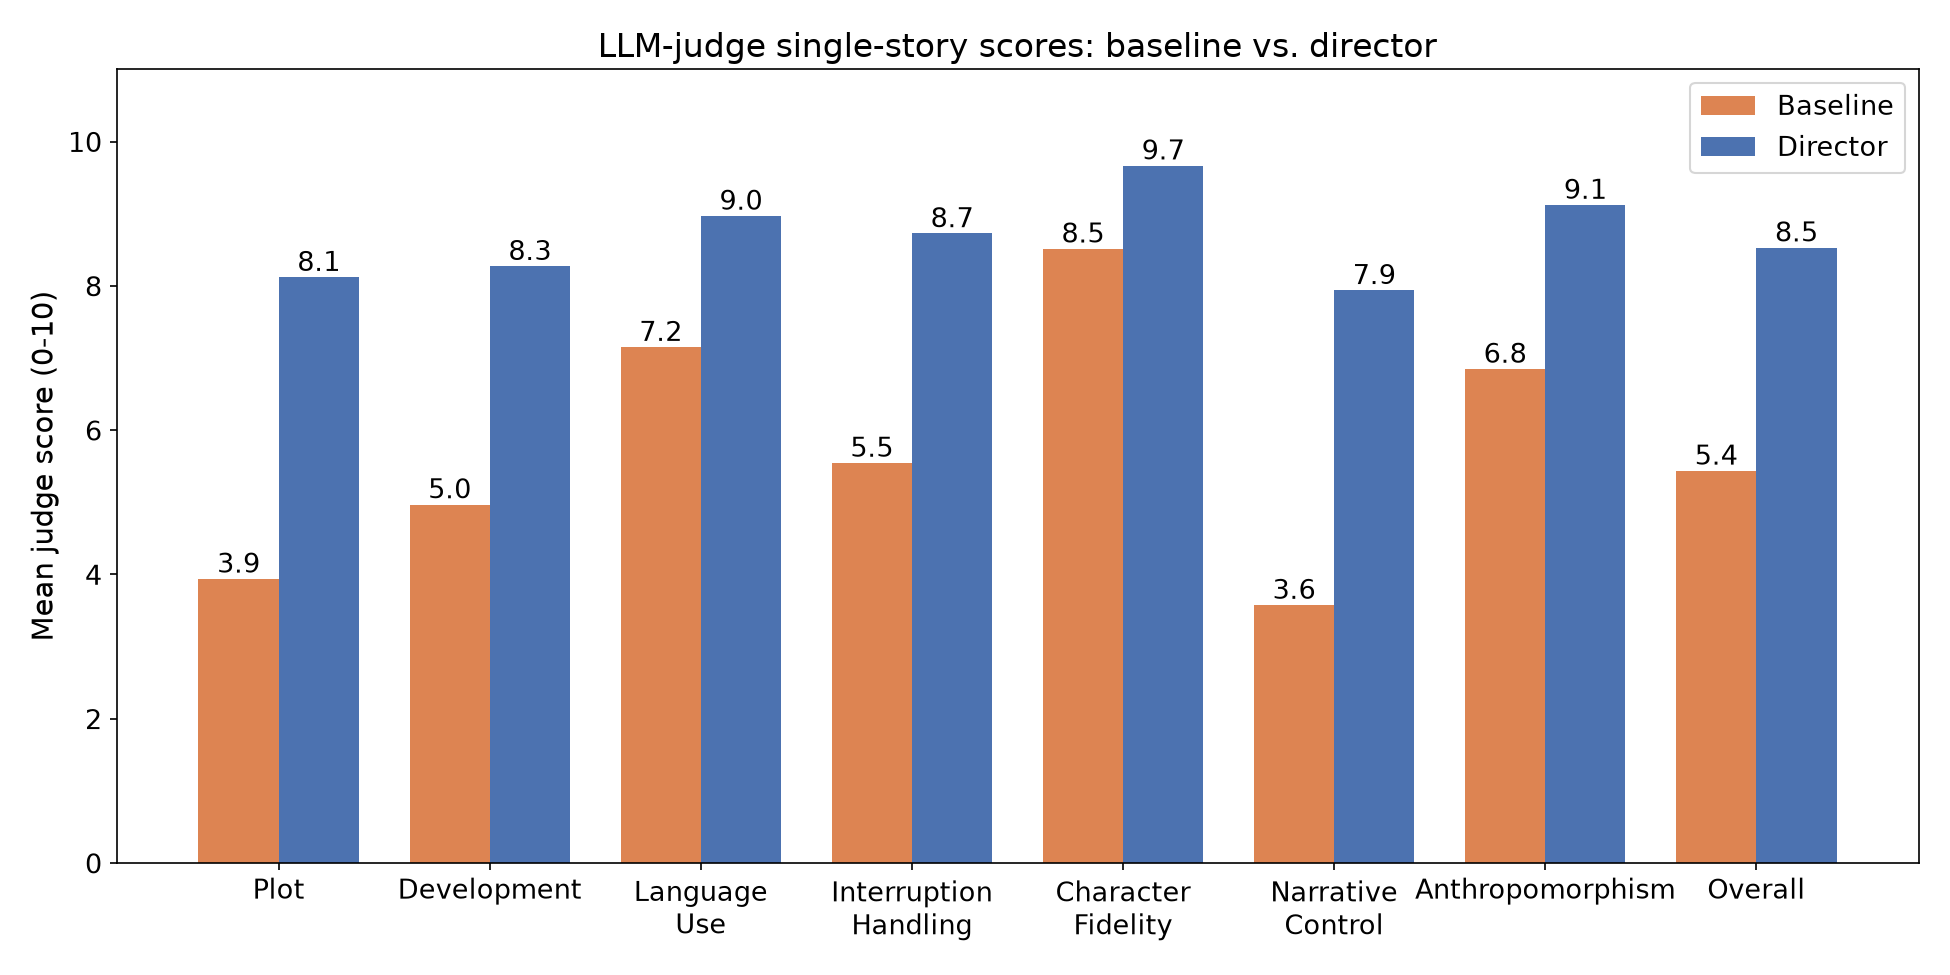
\includegraphics[width=0.95\linewidth]{plots/01_baseline_vs_director_scores_by_metric.png}
\caption{Single-story judge scores, baseline vs.\ director, averaged over all 33 transcript pairs (20 of the 33 director transcripts are post-fix, see above).}
\label{fig:llm-base-metric}
\end{figure}

\begin{table}[htbp]
\centering
\caption{Baseline vs.\ director, mean single-story score per dimension (n=33 pairs).}
\label{tab:llm-base-metric}
\begin{tabular}{lcc}
\toprule
Dimension & Baseline & Director \\
\midrule
Plot                   & 3.94 & 8.12 \\
Development             & 4.97 & 8.27 \\
Language Use            & 7.15 & 8.97 \\
Interruption Handling   & 5.55 & 8.73 \\
Character Fidelity      & 8.52 & 9.67 \\
Narrative Control       & 3.58 & 7.94 \\
Anthropomorphism        & 6.85 & 9.12 \\
Overall                  & 5.44 & 8.53 \\
\bottomrule
\end{tabular}
\end{table}

Director scores higher on every dimension, and now by a much wider margin than either the original draft of this table or the complete-only-fixed version showed. Two dimensions carry the biggest gap: Narrative Control (+4.36) and Plot (+4.18). The judge's own rubric explains why. For Narrative Control it is told to check that the story should make progress through the intended beat structure, that the system should not get stuck in one beat for too long, and that the story should move toward resolution in a coherent way. That wording is close to a direct description of the failure the fix targets. Character Fidelity stays the smallest gap, at +1.15. Staying in character was never baseline's weak point, in the live study or here.

\begin{figure}[htbp]
\centering
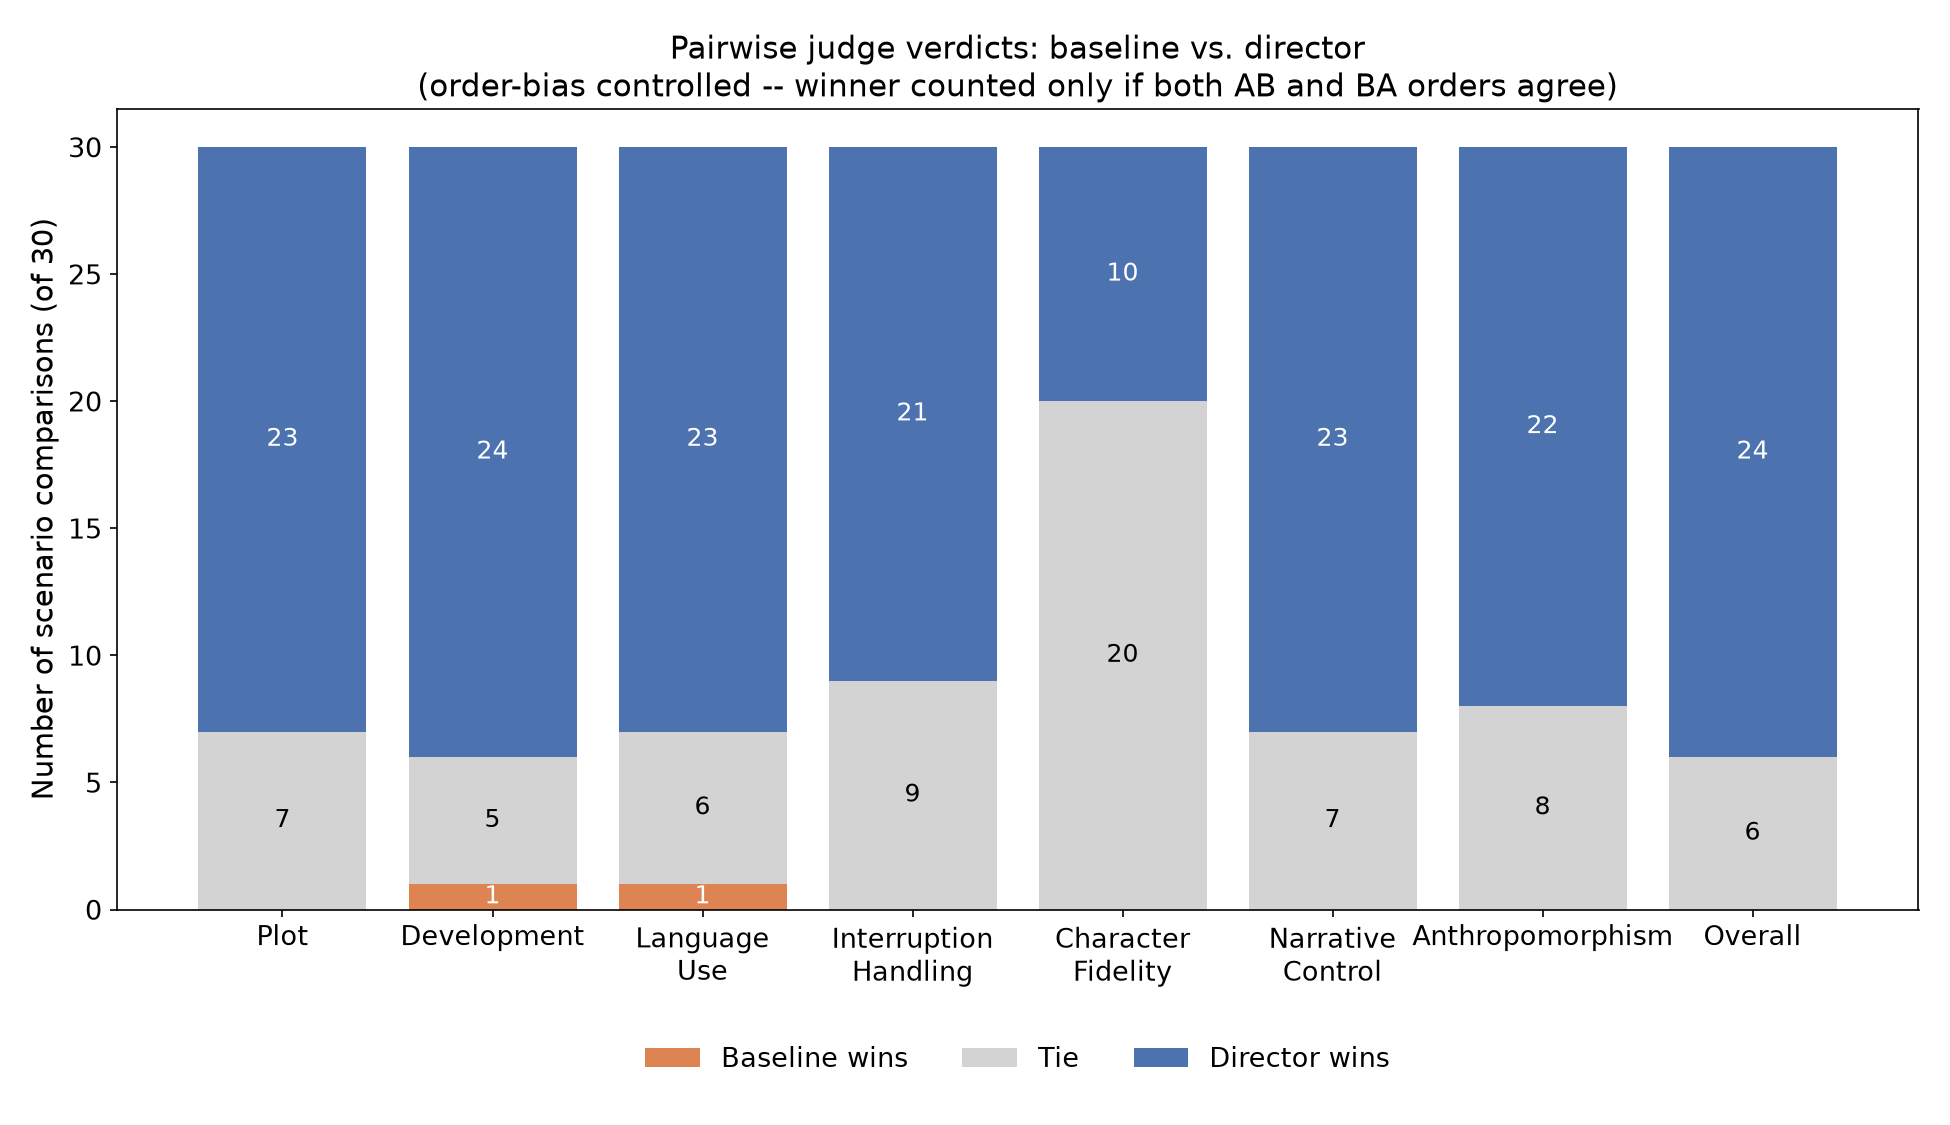
\includegraphics[width=0.95\linewidth]{plots/02_baseline_vs_director_pairwise_wins.png}
\caption{Pairwise verdicts, baseline vs.\ director, order-bias controlled (n=30).}
\label{fig:llm-base-wins}
\end{figure}

The pairwise verdicts in Figure~\ref{fig:llm-base-wins} tell a stricter version of the same story. This figure drops the three legacy Red Riding Hood pilot scenarios that Table~\ref{tab:llm-base-metric} still includes, so it sits at n=30 rather than n=33, matching the scope used everywhere else in this section. A win only counts here if both presentation orders agree on it. Under that rule, baseline wins just 2 of 240 dimension judgments across all 30 pairs. Ties account for 68. Director wins the remaining 170.

Character Fidelity is the one dimension where ties still make up more than half, 20 of 30. On inspection, almost every one of those ties is a \texttt{no\_derailment} scenario. The rubric for Interruption Handling asks the judge to check that the system should handle user interruptions gracefully, and that the story should not get stuck in a loop of interruptions or lose narrative coherence. A no derailment scenario scripts no interruptions at all, so there is nothing for either system to mishandle, and the judge has little basis to pick a winner. Ties on Interruption Handling and Narrative Control never occur on a medium or complete derailment scenario. Once real derailment pressure exists, the two systems separate cleanly enough that both orderings agree almost every time. Where a clear difference does exist, director wins it decisively: 10 to baseline's 0 on Character Fidelity, and similarly one sided margins elsewhere. One assessment, on \texttt{olaf\_lost\_lantern\_adventure\_complete\_derailment}, states the pattern plainly:

\begin{quote}
\small
``Story A struggles with handling interruptions, often getting stuck in a loop and failing to progress the narrative. The character acknowledges the interruptions but does not effectively steer back to the story. Story B handles interruptions gracefully, acknowledging them briefly before steering back to the story. The narrative remains coherent and progresses toward resolution despite frequent interruptions.''
\end{quote}

\begin{figure}[htbp]
\centering
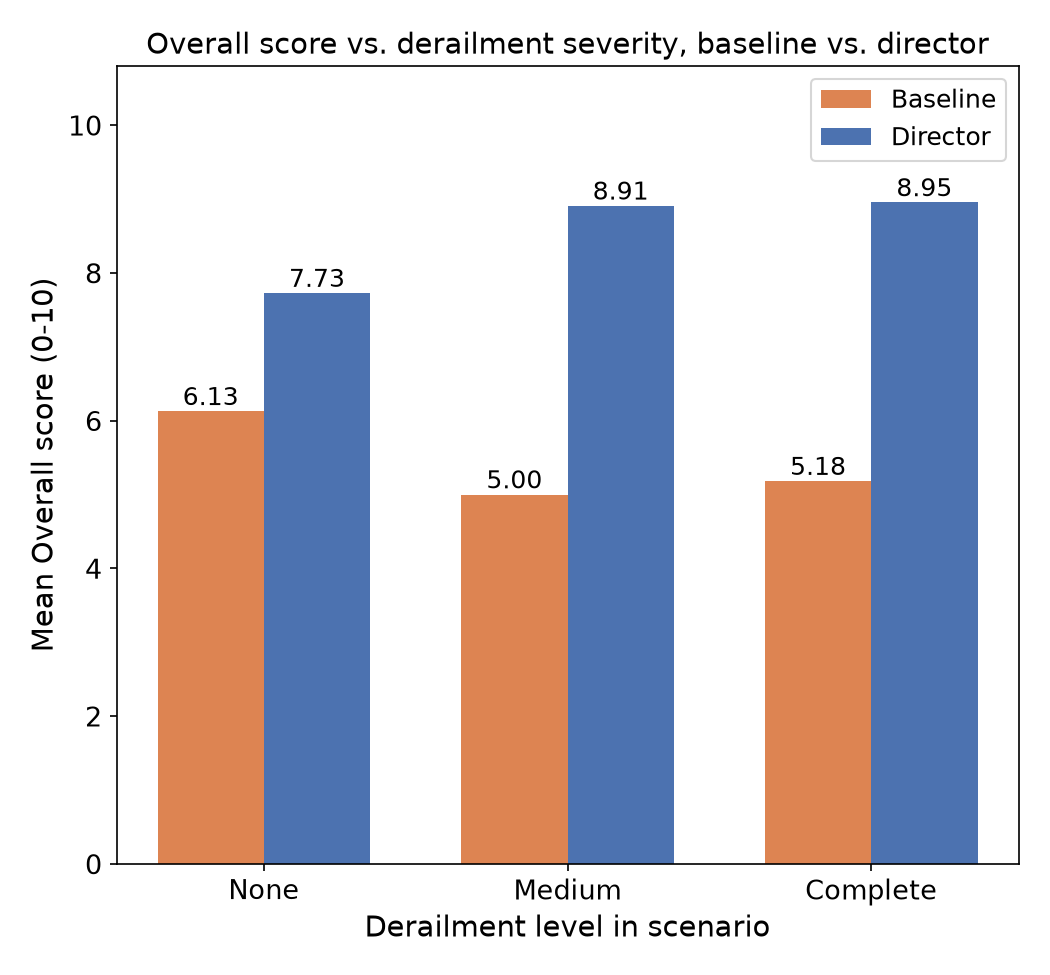
\includegraphics[width=0.6\linewidth]{plots/03_baseline_vs_director_by_derailment_level.png}
\caption{Overall score vs.\ derailment severity, baseline vs.\ director.}
\label{fig:llm-base-derail}
\end{figure}

\begin{table}[htbp]
\centering
\caption{Overall score by derailment level.}
\label{tab:llm-base-derail}
\begin{tabular}{lccc}
\toprule
 & None & Medium & Complete \\
\midrule
Baseline & 6.13 & 5.00 & 5.18 \\
Director & 7.73 & 8.91 & 8.95 \\
\bottomrule
\end{tabular}
\end{table}

Before any fix, director's lead over baseline shrank as derailment got worse. It was 1.60 points at no derailment, down to 0.22 at complete. That was the finding reported in the first draft of this section. With the fix now applied to both Medium and Complete, that pattern has not just disappeared. It has flipped. None, the condition with no injected derailment at all, is now the weakest condition for director: still a 1.60 point lead over baseline, unchanged, because it is still pre fix. Medium and Complete are both fixed now, and both sit far above None, with a 3.91 point lead and a 3.77 point lead that are close to identical. This is not evidence that severity stopped mattering. It confirms, for the second time, that the old bottleneck was never really about how hard the derailment was. It was about whether that specific scenario happened to be generated before or after the fix. The two scenarios still unfixed, \texttt{complete\_derail\_red\_riding\_hood} and \texttt{medium\_derail\_red\_riding\_hood}, score 6.0 and 8.0 on director's Overall. They are the only reason the Complete and Medium averages sit below what their ten fixed scenarios alone would show: 9.25 and 9.00.

\paragraph{Narrative Control and Interruption Handling, read against the rubric.}
Both dimensions are graded on wording that circles the same idea: getting stuck.

\begin{quote}
\small
\textbf{Narrative Control:} The story should make progress through the intended beat structure. The system should not get stuck in one beat for too long. The story should move toward resolution in a coherent way.

\textbf{Interruption Handling:} The system should handle user interruptions gracefully. If the user asks a side question or gives off-topic input, the character should respond naturally and steer back to the story. The story should not derail completely off track because of interruptions. The user should still feel acknowledged. The story should not get stuck in a loop of interruptions or lose narrative coherence. The story should always progress toward the next beat and resolution, even with interruptions.
\end{quote}

\begin{figure}[htbp]
\centering
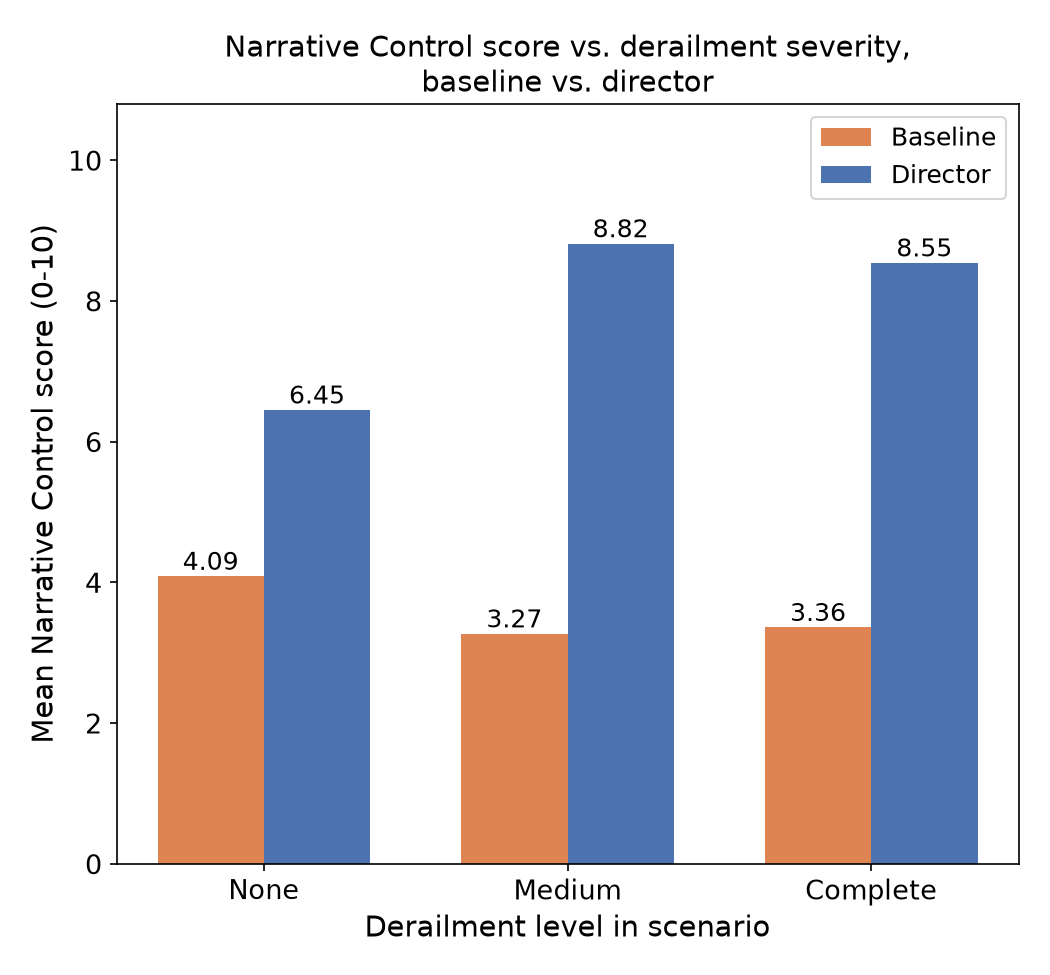
\includegraphics[width=0.6\linewidth]{plots/16_narrative_control_by_derailment_level.png}
\caption{Narrative Control score vs.\ derailment severity, baseline vs.\ director.}
\label{fig:llm-base-nc-derail}
\end{figure}

\begin{figure}[htbp]
\centering
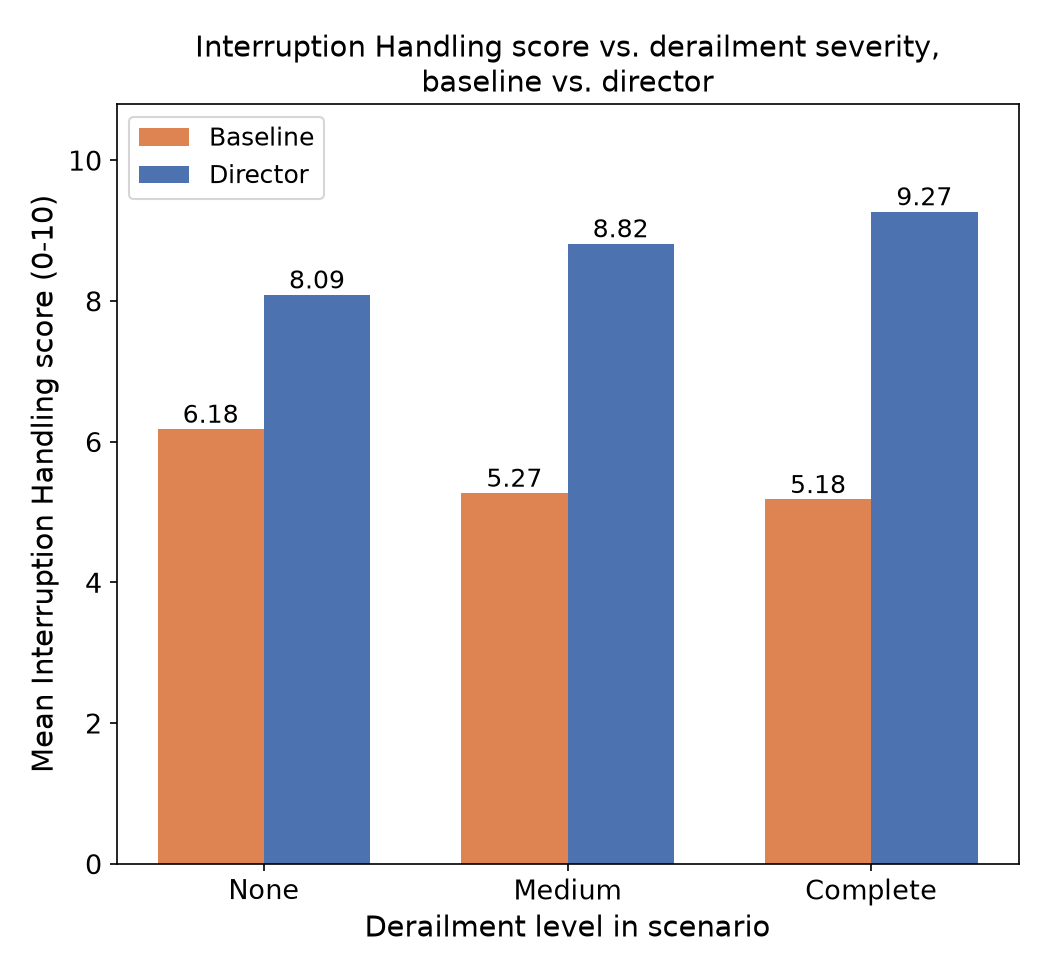
\includegraphics[width=0.6\linewidth]{plots/17_interruption_handling_by_derailment_level.png}
\caption{Interruption Handling score vs.\ derailment severity, baseline vs.\ director.}
\label{fig:llm-base-ih-derail}
\end{figure}

Narrative Control asks whether the plot keeps moving. Interruption Handling asks whether the conversation keeps moving without getting stuck when the user pushes off topic. They are grading close to the same failure from two angles, and Figures~\ref{fig:llm-base-nc-derail} and~\ref{fig:llm-base-ih-derail} move together because of it.

Baseline never had beat tracking to lose, so a fix to beat tracking has nothing to touch. It stays low and roughly flat on both dimensions across all three severities: Narrative Control runs 4.09, 3.27, 3.36 for None, Medium, and Complete; Interruption Handling runs 6.18, 5.27, 5.18. Director tells a different story, and it is the same story as Figure~\ref{fig:llm-base-derail}. At None, still pre fix, director scores 6.45 on Narrative Control and 8.09 on Interruption Handling. At Medium and Complete, both fixed, both dimensions jump to a tight band between 8.5 and 9.3: 8.82 and 8.82 at Medium, 8.55 and 9.27 at Complete. The fix did not make derailment easier in general. It made one specific failure, getting stuck on a beat, mostly disappear wherever it was applied. Since that failure is what both dimensions are built to catch, both jumped together.

\subsection{Director vs.\ CoDi}
\label{sec:llm-codi}

CoDi is an external multi-agent story-generation framework, included as a second point of comparison beyond our own baseline. Where the director-vs-baseline comparison isolates the value of adding a director layer at all, this comparison asks a harder question: how does our specific director design compare to another system built for the same job.

\begin{figure}[htbp]
\centering
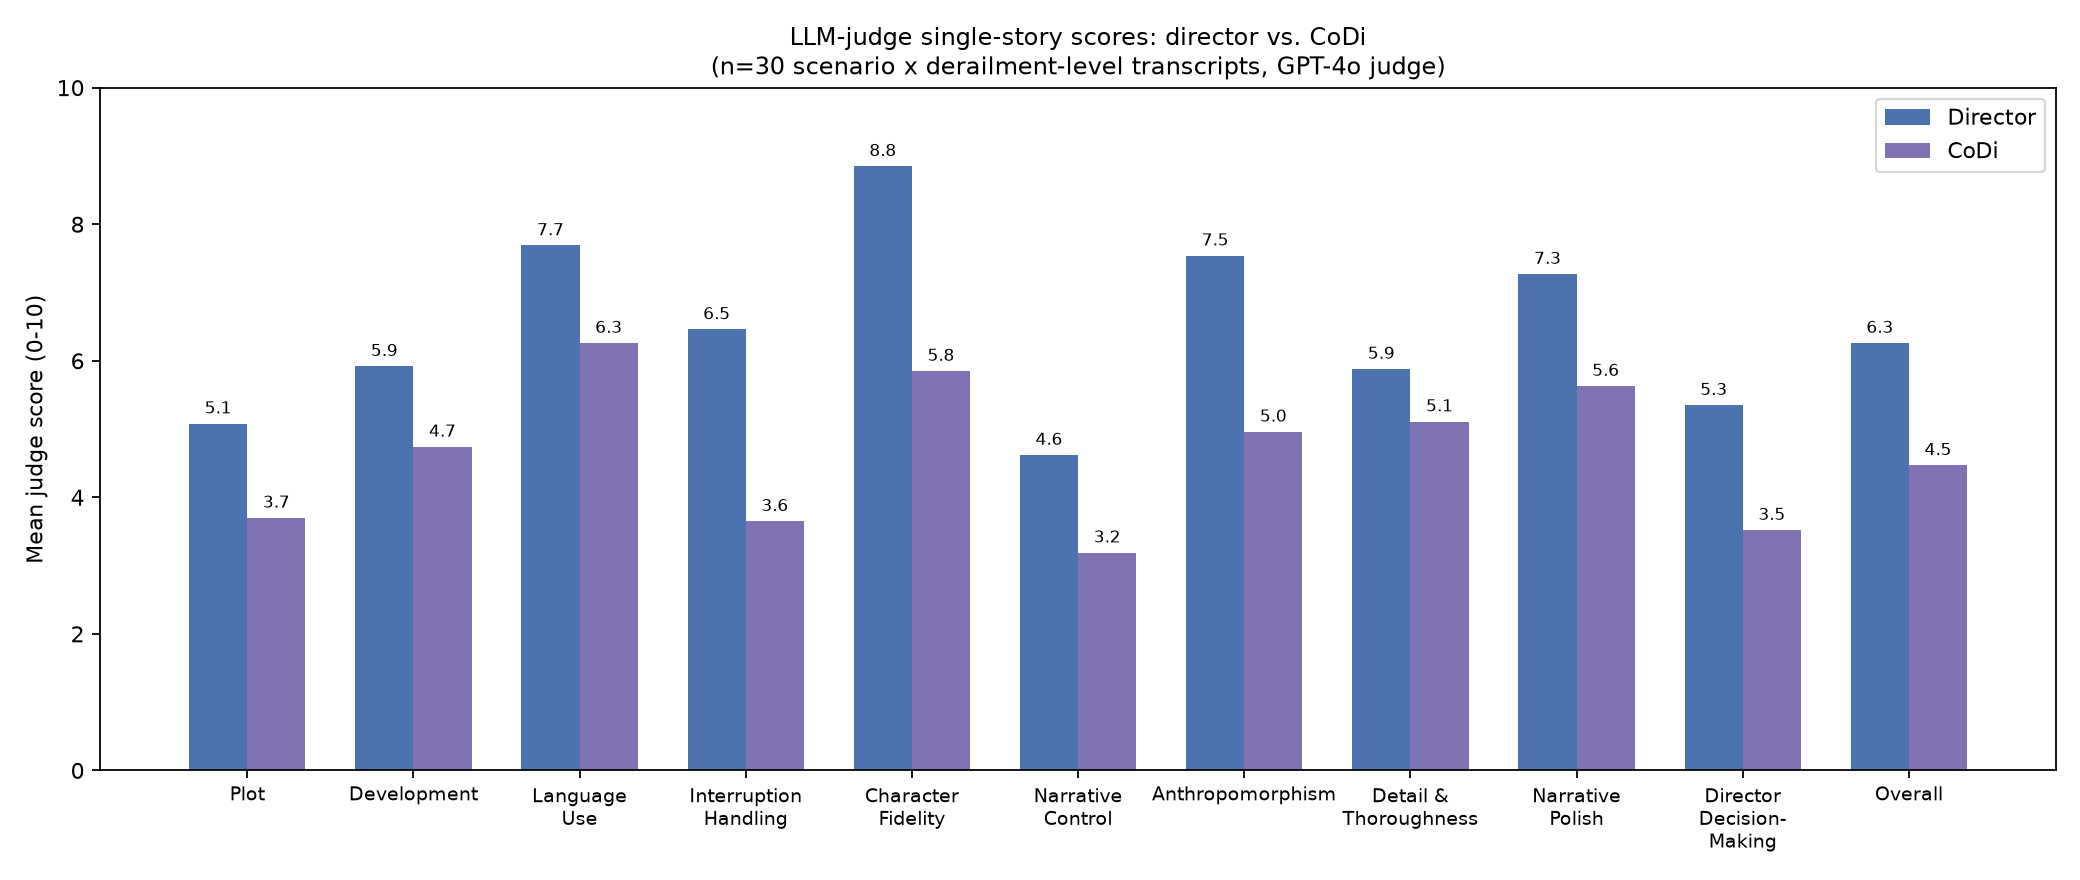
\includegraphics[width=0.95\linewidth]{plots/04_director_vs_codi_scores_by_metric.png}
\caption{Single-story judge scores, director vs.\ CoDi, averaged over 30 transcript pairs.}
\label{fig:llm-codi-metric}
\end{figure}

\begin{table}[htbp]
\centering
\caption{Director vs.\ CoDi, mean single-story score per dimension (n=30 pairs).}
\label{tab:llm-codi-metric}
\begin{tabular}{lcc}
\toprule
Dimension & Director & CoDi \\
\midrule
Plot                       & 5.08 & 3.70 \\
Development                 & 5.92 & 4.74 \\
Language Use                & 7.69 & 6.26 \\
Interruption Handling       & 6.46 & 3.65 \\
Character Fidelity          & 8.85 & 5.85 \\
Narrative Control           & 4.62 & 3.19 \\
Anthropomorphism            & 7.54 & 4.96 \\
Detail \& Thoroughness       & 5.88 & 5.11 \\
Narrative Polish            & 7.27 & 5.63 \\
Director Decision-Making    & 5.35 & 3.52 \\
Overall                      & 6.26 & 4.47 \\
\bottomrule
\end{tabular}
\end{table}

Director scores higher on every dimension here too, including the three added specifically to give CoDi's multi-agent planning a fair shot (Detail \& Thoroughness, Narrative Polish, Director Decision-Making). The margin is largest on Character Fidelity (+3.00) and Interruption Handling (+2.81) — the two dimensions most directly tied to staying in character while being interrupted.

\begin{figure}[htbp]
\centering
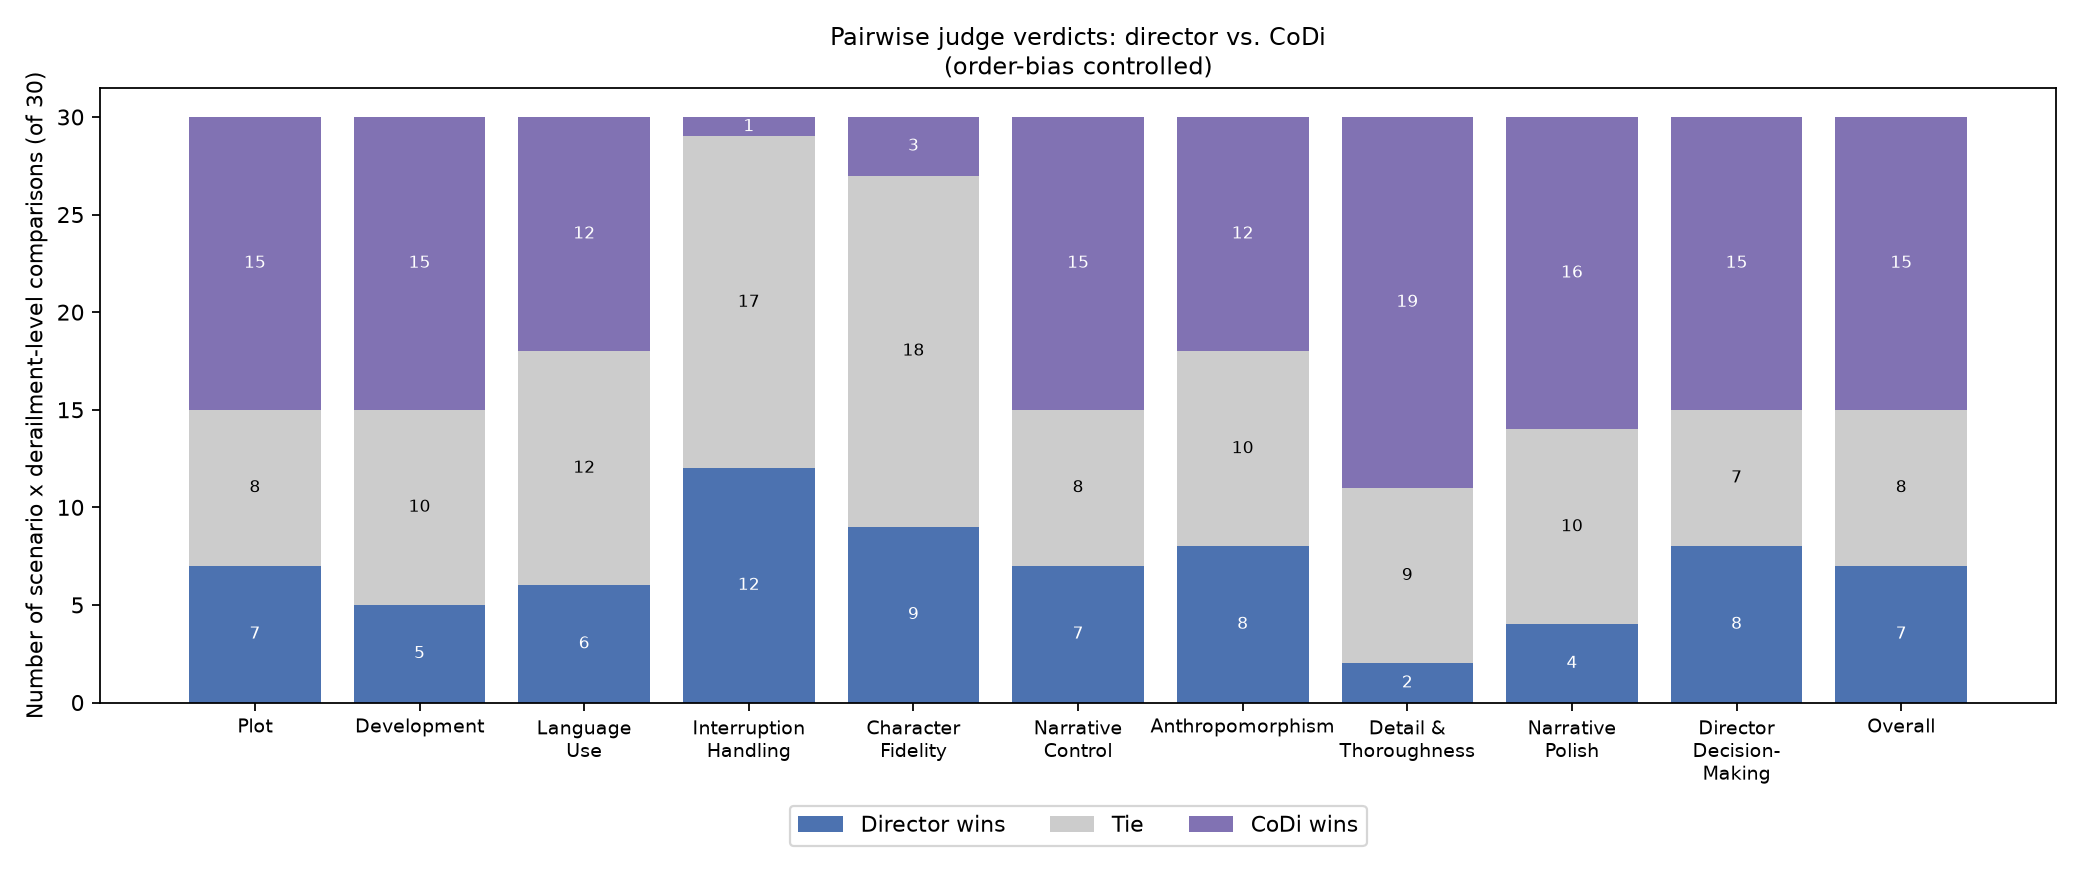
\includegraphics[width=0.95\linewidth]{plots/05_director_vs_codi_pairwise_wins.png}
\caption{Pairwise verdicts, director vs.\ CoDi, order-bias controlled (n=30).}
\label{fig:llm-codi-wins}
\end{figure}

The pairwise verdicts complicate this picture in an interesting way. CoDi wins outright on Plot, Development, Narrative Control, Detail \& Thoroughness, Narrative Polish, and Director Decision-Making — the dimensions about craft and planning. Director wins outright on exactly two: Interruption Handling (12 wins vs.\ CoDi's 1, 17 ties) and Character Fidelity (9 vs.\ 3, 18 ties). One assessment states the trade-off directly:

\begin{quote}
\small
``System A [director] effectively manages interruptions, keeping the narrative on track, albeit at the cost of progression.'' \\
``The narrative includes rich descriptions and thorough scene development, providing a comprehensive and immersive experience'' [System B, CoDi, on Detail \& Thoroughness].
\end{quote}

So the two systems specialize. CoDi, with more planning overhead, produces more detailed, better-plotted prose when left alone. Director is worse at that, but it is built specifically to keep a live, interruptible conversation on track without breaking character — and on exactly that axis, it beats CoDi more decisively than on anything else. Given that interruption handling is the central problem this thesis addresses, this is the more relevant result of the two, even though it is not where director wins the most dimensions.

\subsection{Time-Budget Ablation}
\label{sec:llm-time}

The live user study tests one time budget (5 minutes) against no budget at all. Here we test four fixed budgets — 0.5, 2, 5, and 10 minutes — against each other and against the unconstrained director, all on the same 30 scenarios, using two rule-based structural metrics (no LLM involved) alongside the judge's qualitative score.

\begin{figure}[htbp]
\centering
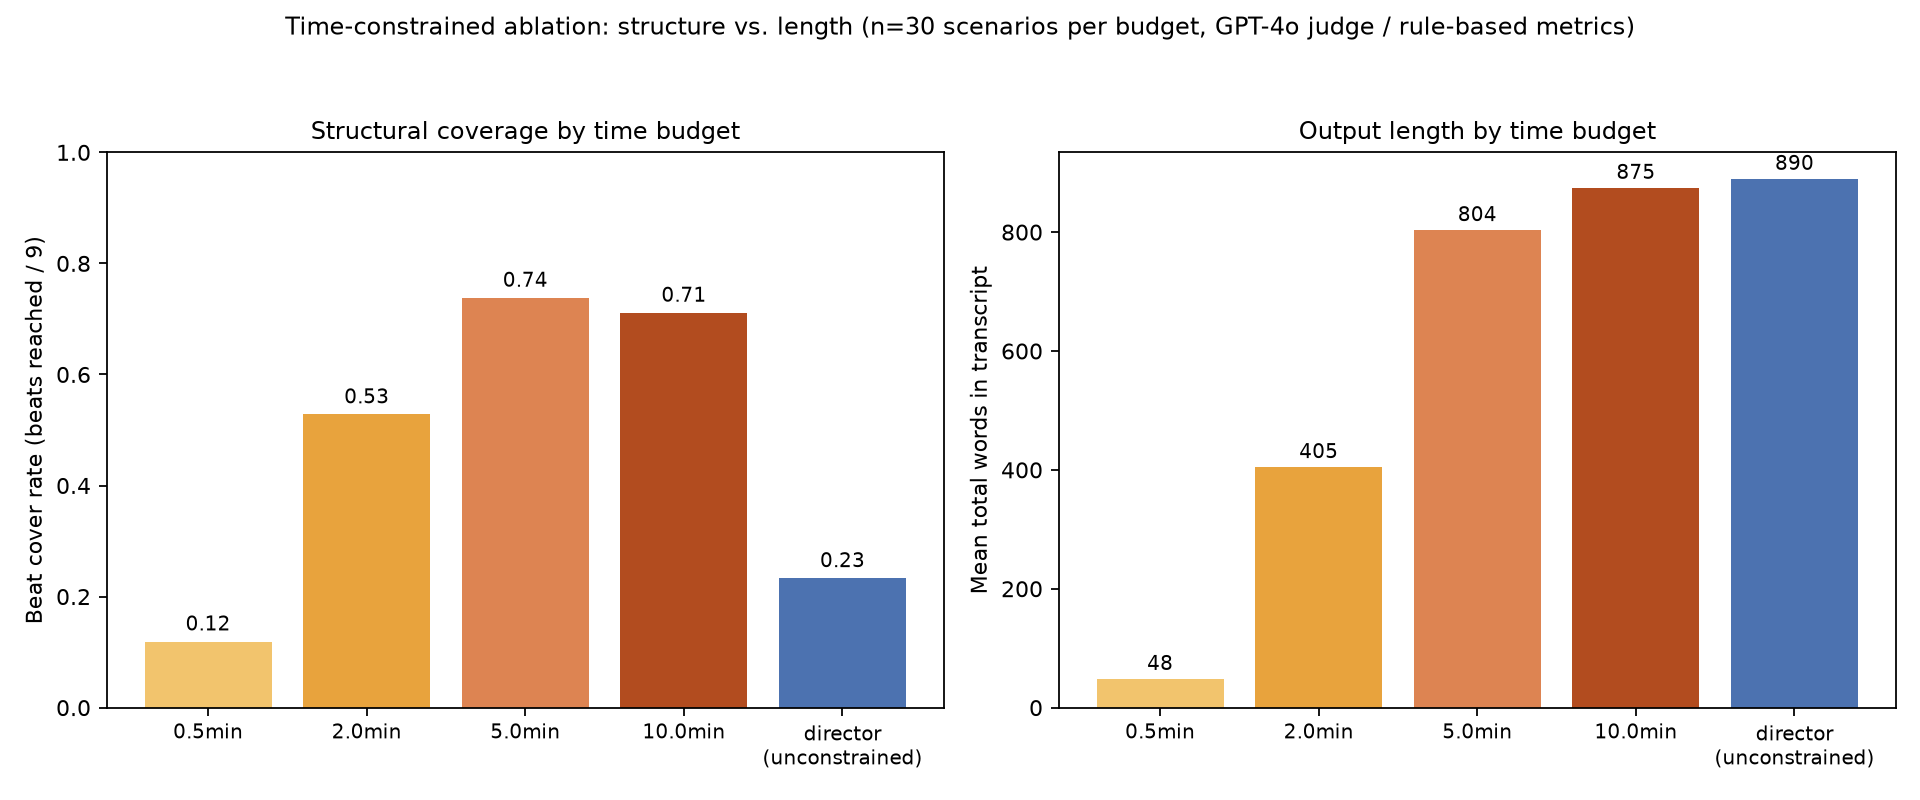
\includegraphics[width=0.95\linewidth]{plots/06_time_constrained_coverage_and_length.png}
\caption{Beat coverage and output length across time budgets (n=30 scenarios per budget).}
\label{fig:llm-time-coverage}
\end{figure}

\begin{table}[htbp]
\centering
\caption{Structural metrics by time budget.}
\label{tab:llm-time-metrics}
\begin{tabular}{lccccc}
\toprule
 & 0.5min & 2.0min & 5.0min & 10.0min & Director (unconstrained) \\
\midrule
Beat cover rate      & 0.12 & 0.53 & 0.74 & 0.71 & 0.23 \\
Total words (mean)   & 48   & 405  & 804  & 875  & 890 \\
Truncated (share)    & 100\% & 100\% & 100\% & 100\% & 100\% \\
\bottomrule
\end{tabular}
\end{table}

Beat coverage rises sharply from 0.5 to 5 minutes, then \emph{plateaus and slightly drops} from 5 to 10 minutes (0.74 to 0.71) — more time past a point does not buy more structure. The unconstrained director is the extreme case: it produces the most words of any condition (890, more even than the 10-minute budget) but covers the fewest beats (0.23) — almost the same wasteful pattern the live study found, where the unconstrained round rarely reached an ending despite generating plenty of text. And every single transcript in this ablation, at every budget including 10 minutes, is flagged as truncated: none of them cleanly complete their final beat. A time budget changes how much of the story gets told, not whether it finishes cleanly.

\begin{figure}[htbp]
\centering
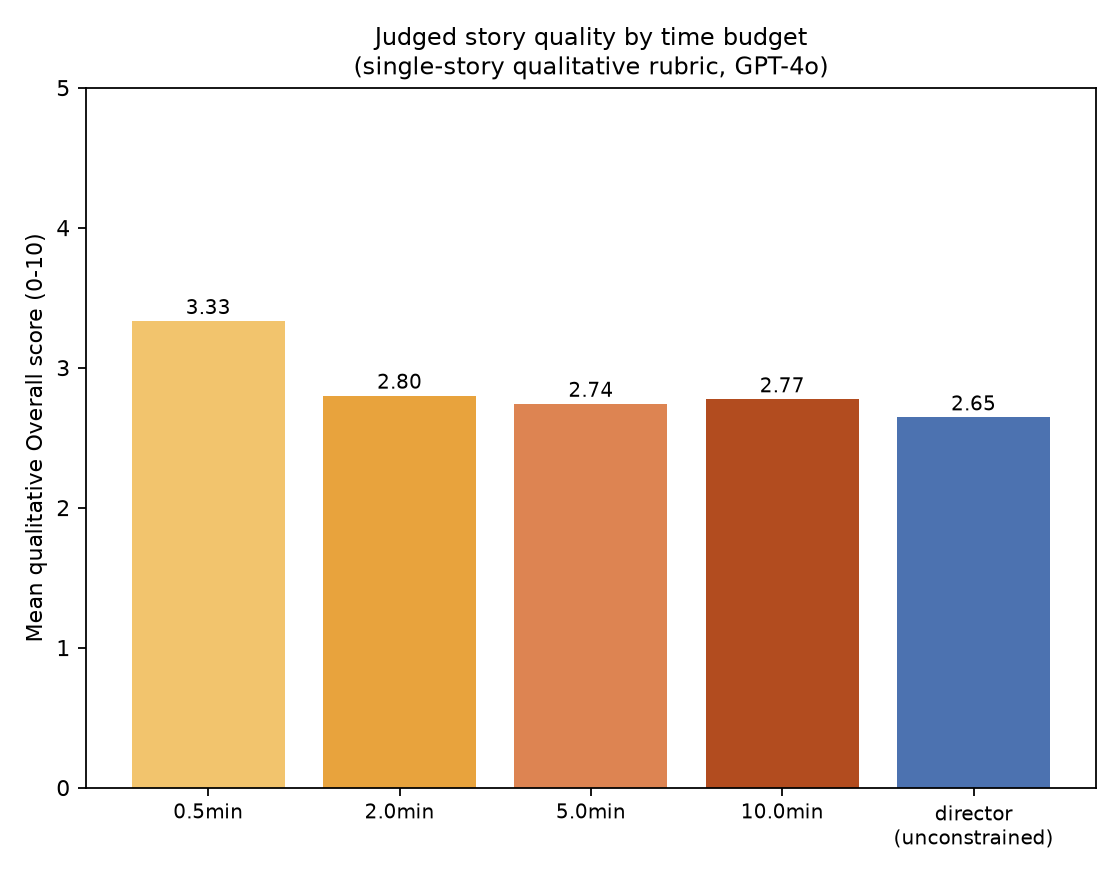
\includegraphics[width=0.65\linewidth]{plots/07_time_constrained_qualitative_overall.png}
\caption{Judged story quality (single-story Overall) by time budget.}
\label{fig:llm-time-qual}
\end{figure}

The judged quality score (Figure~\ref{fig:llm-time-qual}) runs the other way: it is \emph{highest} at 0.5 minutes (3.33) and lowest for the unconstrained director (2.65), with 2--10 minutes clustered in between. This looks backwards until read alongside Table~\ref{tab:llm-time-metrics}: a 0.5-minute story is a single short scene, with almost nothing in it to go wrong — no time to lose the thread, repeat itself, or mishandle an interruption. The judge was explicitly instructed not to penalize a short story for being short, and a near-empty story is easy to rate as clean. Longer, more structurally complete stories have more surface area for judged flaws, even though they objectively cover more of the plot. We read this as a limitation of a single-story quality score under a time constraint, not as evidence that shorter is actually better — the beat-coverage numbers in Table~\ref{tab:llm-time-metrics} are the more trustworthy measure of what these budgets actually accomplish.

Finally, embedding-based cosine similarity between transcripts at different budgets (Table~\ref{tab:llm-time-sim}) shows budgets close in length stay close in content (5 vs.\ 10 minutes: 0.91) while the 0.5-minute condition diverges from everything else (0.66--0.69) — consistent with it being a different, much shorter story rather than a compressed version of the same one.

\begin{table}[htbp]
\centering
\caption{Pairwise cosine similarity between transcripts at different time budgets, averaged across scenarios.}
\label{tab:llm-time-sim}
\begin{tabular}{lccccc}
\toprule
 & 0.5min & 2.0min & 5.0min & 10.0min & Director \\
\midrule
0.5min    & 1.00 & 0.76 & 0.68 & 0.69 & 0.67 \\
2.0min    & 0.76 & 1.00 & 0.88 & 0.86 & 0.84 \\
5.0min    & 0.68 & 0.88 & 1.00 & 0.91 & 0.88 \\
10.0min   & 0.69 & 0.86 & 0.91 & 1.00 & 0.89 \\
Director  & 0.67 & 0.84 & 0.88 & 0.89 & 1.00 \\
\bottomrule
\end{tabular}
\end{table}

\subsection{Cross-Checking the Live Study: Frozen and Cinderella}
\label{sec:llm-vs-study}

The comparisons above pool 30--33 scenarios the live study never saw, which is the point of running an automated judge at all. But it is also possible to ask the judge about the two exact stories 28 participants actually played and check whether an automated GPT-4o judge and 14 live humans notice the same thing.

For this cross-check, the automated side uses each story's \emph{complete-derailment} scenario variant, not the plain no-derailment one used elsewhere by default. The live study's welcome screen explicitly instructed participants to ``go off-topic, ask him something random, bring up a different subject'' every round (Section~\ref{sec:design}), so every live rating already reflects a story under sustained, deliberate derailment pressure. The complete-derailment automated variant is the one built to match that: it scripts the heaviest, most persistent stream of off-topic and adversarial user turns in the suite, unlike no-derailment, which scripts none. Comparing the live numbers against the no-derailment judge run, as an earlier draft of this section did, was comparing a derailment-stress-tested human condition against a judge condition with no derailment in it at all; complete-derailment is the honest match.

Story 1 (Section~\ref{sec:story1}) is \texttt{olaf\_retells\_frozen\_1\_complete\_derailment}, director vs.\ baseline. Story 2 (Section~\ref{sec:story2}) is \texttt{olaf\_retells\_cinderella\_complete\_derailment}, director vs.\ a time-constrained director. Each condition below is generated and judged five separate times, and the numbers reported are the mean of those five runs, not one transcript. That is still five runs per condition, not 14 paired ratings, so this remains a case study cross check on the aggregate results above, not an independently powered result on its own.

\subsubsection{Mapping the Questionnaire to the Judge Rubric}
\label{sec:llm-vs-study-mapping}

The two evaluators do not share a common instrument -- the live study asks 5-point Likert questions (Table~\ref{tab:instrument}), the judge scores an 8-dimension rubric (Table~\ref{tab:rubric}) 0--10. Table~\ref{tab:question-mapping} sets out the closest correspondence between the two before comparing them directly in the subsections below.

\begin{table}[htbp]
\centering
\caption{Live-study questionnaire items mapped to the closest LLM-judge rubric dimension(s).}
\label{tab:question-mapping}
\small
\begin{tabular}{p{2.4cm}p{5.6cm}p{4.3cm}p{1.6cm}}
\toprule
Question & Wording & Closest judge dimension(s) & Fit \\
\midrule
Q1 & Story felt coherent, clear narrative arc & Plot & Direct \\
Q2 & Olaf stayed in character & Character Fidelity & Direct \\
Q4 & Engaging / enjoyable & \emph{No direct match} (loosely: Language Use, Anthropomorphism) & Weak \\
Q5 & Overall rating & Overall & Direct \\
Q6-resist & Stayed on track despite derailment & Interruption Handling (primary), Narrative Control (secondary) & Direct, split \\
Q8-ending & Ending satisfying (Story 2 only) & \emph{No BASE match}; closest is the time-ablation's Setup/Payoff Preservation & Weak \\
Q10-natural & Felt natural, not scripted (Story 2 only) & Language Use, Anthropomorphism & Loose \\
Q-pacing & Well-paced / rushed / cut short & \emph{No BASE match}; closest are the time-ablation's Three-Act Balance, Transition Quality & Loose \\
\bottomrule
\end{tabular}
\end{table}

The five core measures used in the comparisons below (Q1, Q2, Q4, Q5, Q6-resist) split cleanly into two groups. Q1, Q2, and Q5 have a clean one-to-one judge dimension (Plot, Character Fidelity, Overall respectively), so a live-vs-judge comparison on those three is comparing genuinely equivalent constructs. Q6-resist has no single equivalent -- it spans both Interruption Handling (does the character acknowledge and recover from the interruption) and Narrative Control (does the story keep moving toward its beats regardless) -- so the discussion below reads it against both rather than picking one. Q4 (engagement) is the weakest link: no judge dimension isolates subjective enjoyment, so agreement or disagreement on that measure specifically should be read with more caution than the other four.

\subsubsection{Frozen}

\begin{table}[htbp]
\centering
\caption{Frozen (\texttt{olaf\_retells\_frozen\_1\_complete\_derailment}), the exact story served in the live study under sustained derailment: judge score, baseline vs.\ director, mean of 5 runs per condition.}
\label{tab:llm-frozen-case}
\begin{tabular}{lcc}
\toprule
Dimension & Baseline & Director \\
\midrule
Plot                    & 4.0 & 9.0  \\
Development             & 5.2 & 8.4  \\
Language Use            & 7.2 & 9.2  \\
Interruption Handling   & 5.6 & 9.0  \\
Character Fidelity      & 8.4 & 10.0 \\
Narrative Control       & 3.2 & 9.0  \\
Anthropomorphism        & 7.0 & 9.2  \\
Overall                 & 5.4 & 9.0  \\
\bottomrule
\end{tabular}
\end{table}

\begin{figure}[htbp]
\centering
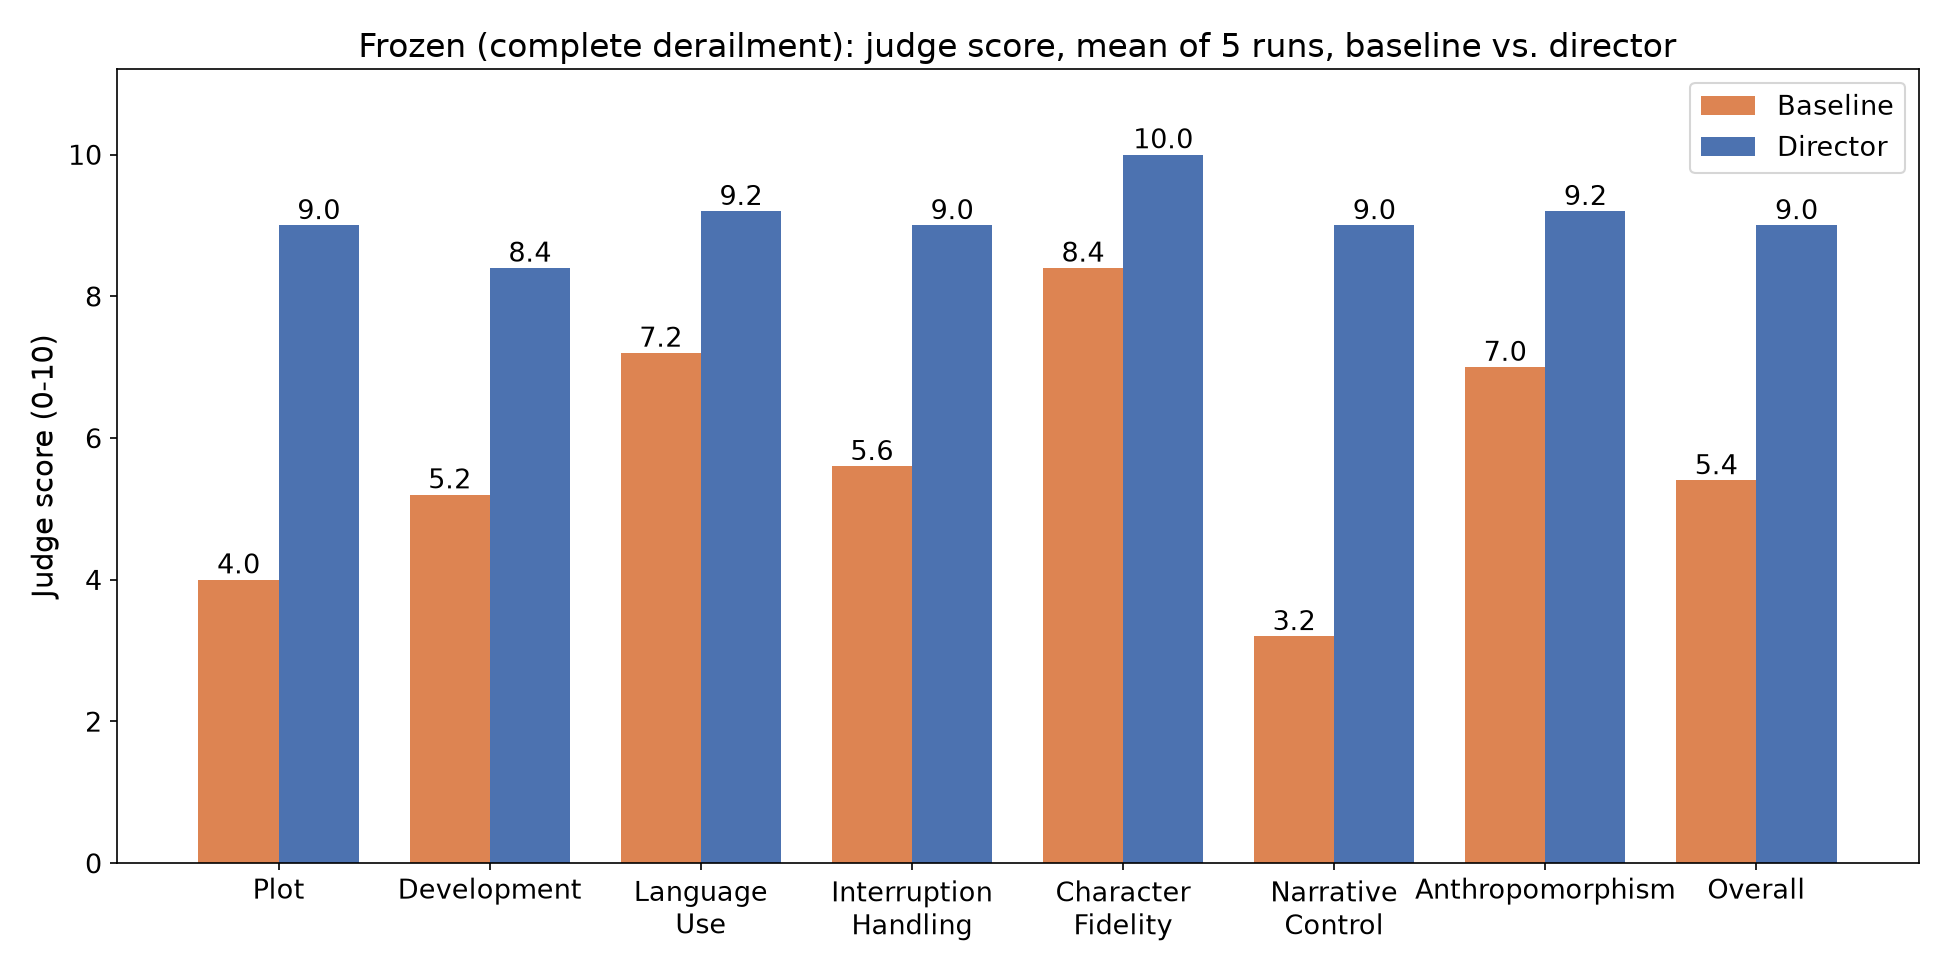
\includegraphics[width=0.95\linewidth]{plots/14_frozen_case_study_complete_derailment.png}
\caption{Frozen, complete derailment: judge score, baseline vs.\ director, mean of 5 runs per condition.}
\label{fig:llm-frozen-case}
\end{figure}

\begin{figure}[htbp]
\centering
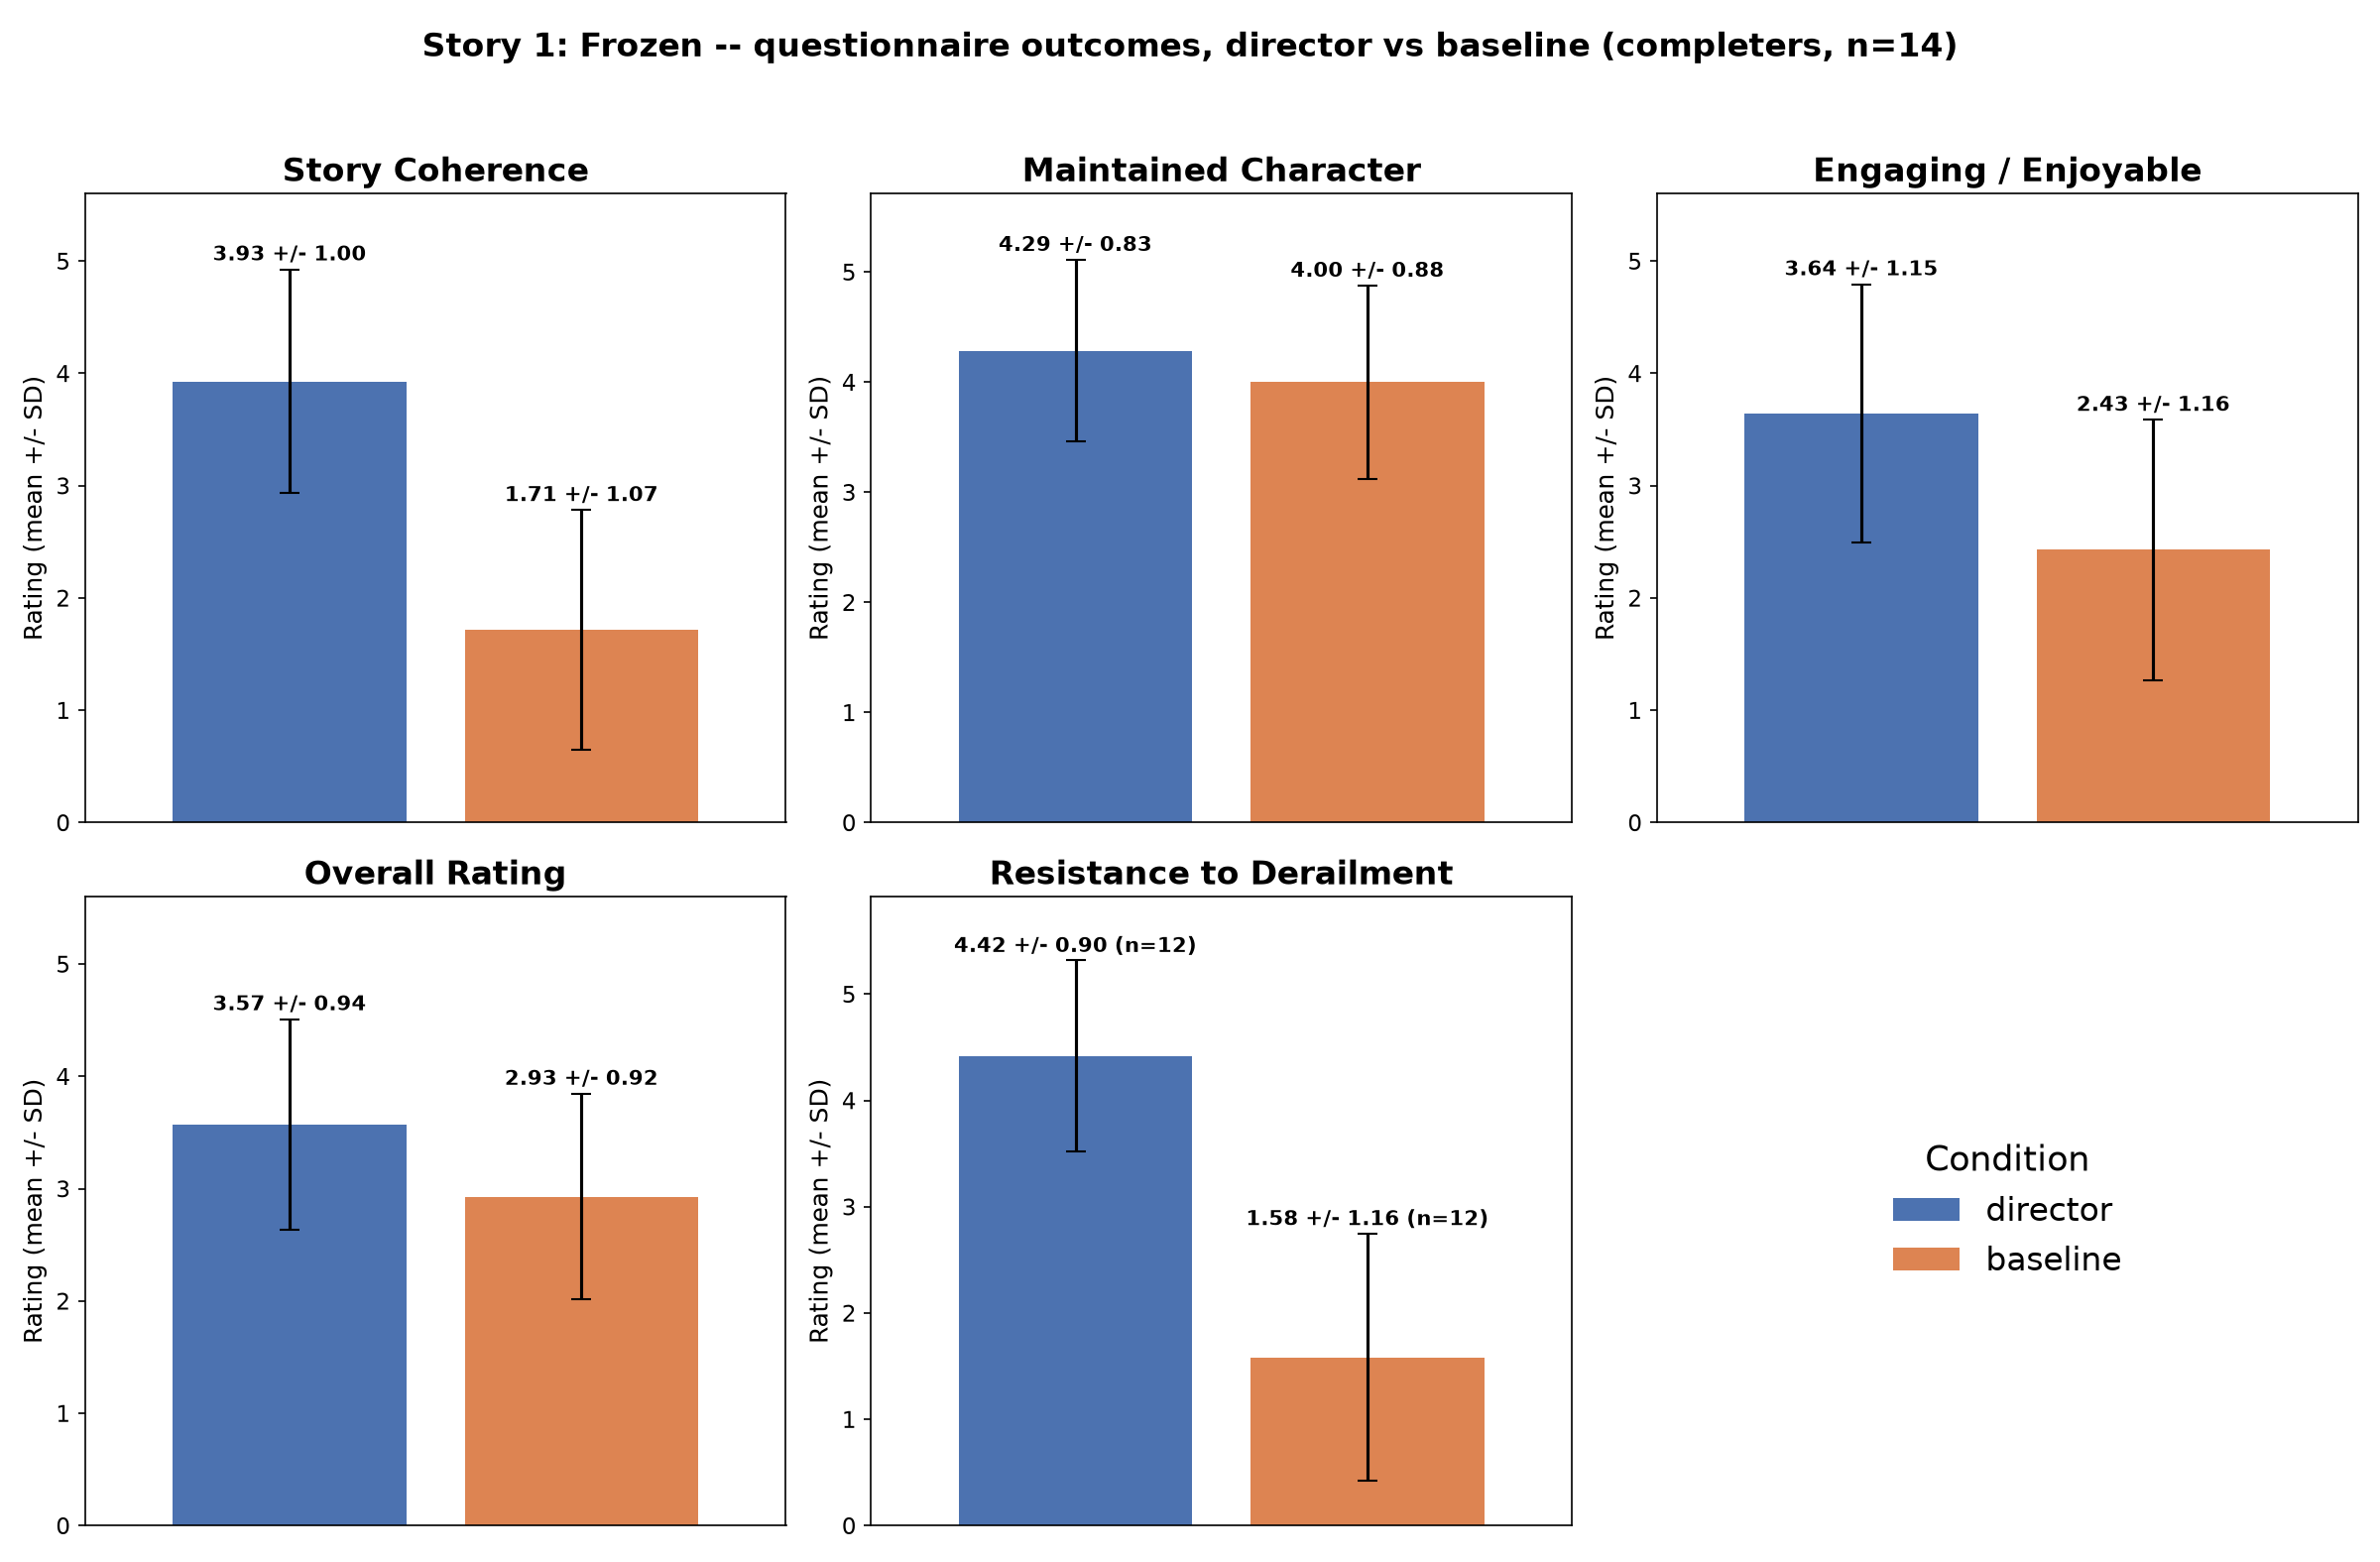
\includegraphics[width=0.95\linewidth]{plots/13_story1_all_measures.png}
\caption{For comparison: the live-study version of the same comparison, director vs.\ baseline on Frozen, all completers ($n$=14; reproduced from Figure~\ref{fig:story1-all}).}
\label{fig:llm-frozen-live}
\end{figure}

Under sustained derailment, baseline collapses hardest on exactly the dimensions Table~\ref{tab:story1} flags. Narrative Control (3.2) is the lowest score baseline gets anywhere in this table, and it is also the biggest judge gap, at +5.8. Plot is close behind at +5.0. Character Fidelity is the smallest gap, at +1.6. That is the same shape as the live result. Participants rated Coherence and derailment resistance as the two measures with the largest, most significant director over baseline gaps, both $p \le 0.002$, while Stayed in Character (Q2) was the one measure with no real difference, 4.29 vs.\ 4.00, \pval{0.40}. Two independent evaluators looked at a comparable derailment load, one made of 14 humans on a 5 point scale and one an automated judge averaging five runs on a 10 point scale, and landed on the same conclusion. Under pressure to derail, baseline's problem is the plot, not the persona.

\subsubsection{Cinderella}

The automated time-budget ablation (Section~\ref{sec:llm-time}) was run at 0.5, 2, 5, and 10 minutes. The live study's time-constrained condition used a 3-minute budget (see the correction below). There is no exact match, so this section uses the 5-minute budget as the closest grid point, alongside baseline and the unconstrained director for context, all on the complete-derailment variant.

\begin{table}[htbp]
\centering
\caption{Cinderella (\texttt{olaf\_retells\_cinderella\_complete\_derailment}), the exact story served in the live study under sustained derailment: judge score, mean of 5 runs per condition. 5 min is the closest automated grid point to the live study's 3-minute time-constrained condition.}
\label{tab:llm-cinderella-case}
\begin{tabular}{lccc}
\toprule
Dimension & Baseline & Director & 5 min \\
\midrule
Plot                    & 4.8 & 9.0  & 8.8  \\
Development             & 5.8 & 8.4  & 8.6  \\
Language Use            & 7.6 & 9.2  & 9.4  \\
Interruption Handling   & 5.6 & 9.8  & 9.4  \\
Character Fidelity      & 8.6 & 10.0 & 10.0 \\
Narrative Control       & 4.4 & 9.0  & 8.8  \\
Anthropomorphism        & 7.4 & 9.2  & 9.6  \\
Overall                 & 6.2 & 9.1  & 9.1  \\
\bottomrule
\end{tabular}
\end{table}

\begin{figure}[htbp]
\centering
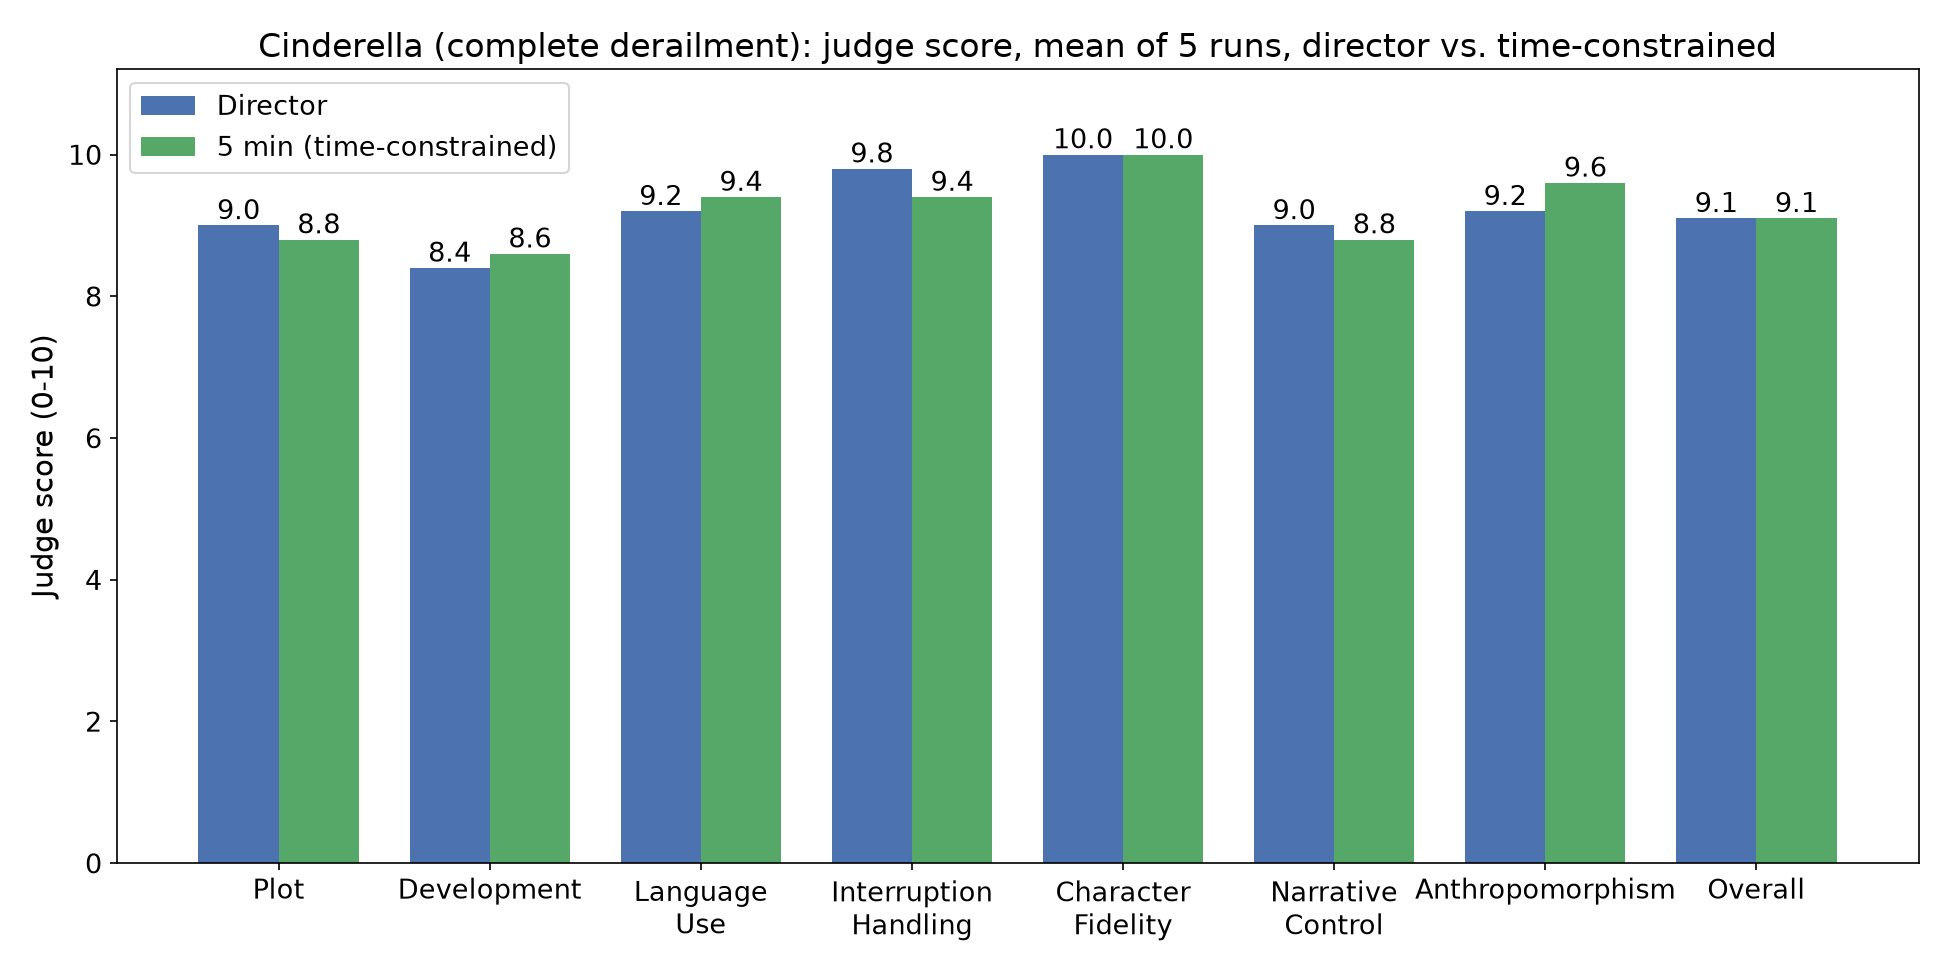
\includegraphics[width=0.95\linewidth]{plots/15_cinderella_case_study_complete_derailment.png}
\caption{Cinderella, complete derailment: judge score, director vs.\ the 5-minute time-constrained budget, mean of 5 runs per condition. Baseline is omitted from the figure but reported in Table~\ref{tab:llm-cinderella-case}.}
\label{fig:llm-cinderella-case}
\end{figure}

\begin{figure}[htbp]
\centering
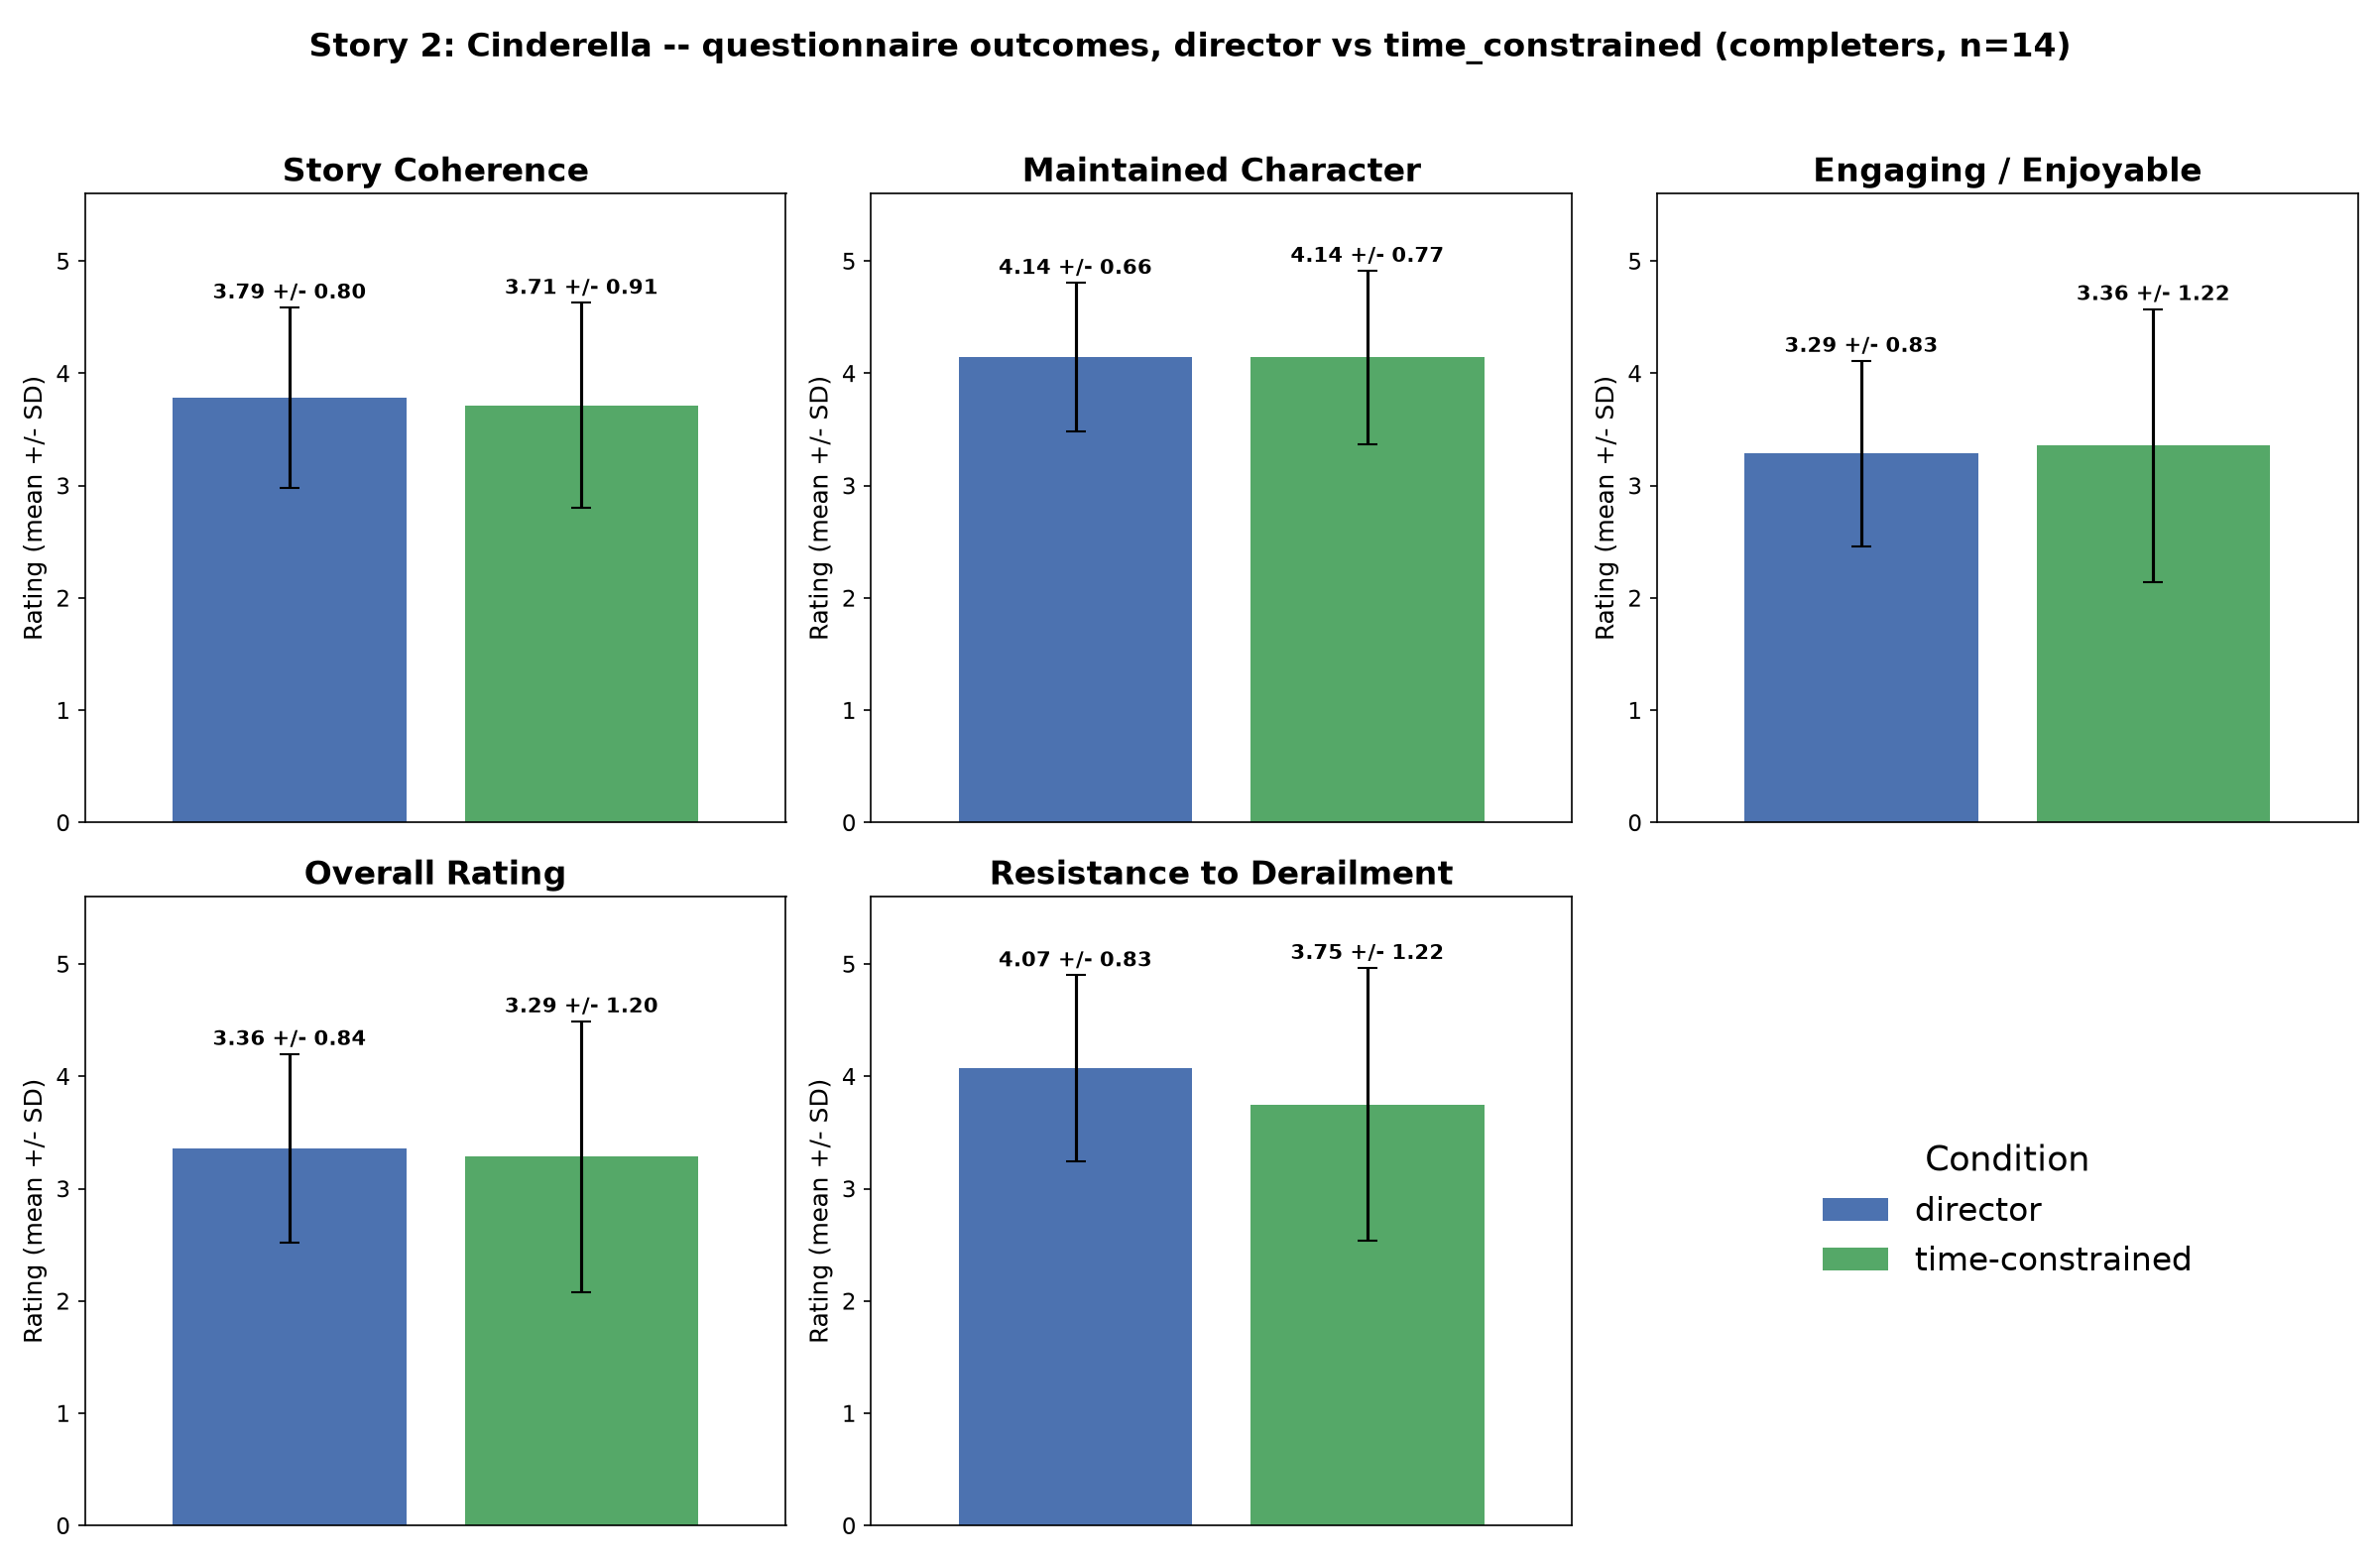
\includegraphics[width=0.95\linewidth]{plots/15_story2_all_measures.png}
\caption{For comparison: the live-study version of the same comparison, director vs.\ time-constrained on Cinderella, all completers ($n$=14; reproduced from Figure~\ref{fig:story2-all}).}
\label{fig:llm-cinderella-live}
\end{figure}

Two things line up with Table~\ref{tab:story2}. First, director vs.\ baseline on this specific story reproduces the same pattern as Frozen under derailment. Narrative Control has the biggest gap, at +4.6. Interruption Handling and Plot are close behind, both at +4.2. Character Fidelity is again the smallest gap, at +1.4. Second, and more relevant to Section~\ref{sec:story2}'s actual comparison: director and the 5-minute budget land within half a point of each other on every dimension, and tie exactly on Character Fidelity and Overall. Neither system beats the other consistently: director edges ahead on Interruption Handling and Narrative Control, the 5-minute budget edges ahead on Development and Anthropomorphism, and the rest are a wash. That is the judge's version of Table~\ref{tab:story2}'s result that none of the five live measures differ significantly between director and time-constrained, all \pval{\ge 0.40}. Both evaluators agree that, even under sustained derailment, adding a time budget on top of the director costs almost nothing, unlike swapping the director out for baseline entirely.

\subsubsection{Data-quality notes from building this cross-check}

Two issues surfaced while pulling the numbers above, both worth recording since they affect how much weight this section's numbers -- and by extension the pooled tables earlier in this section -- should be given.

\begin{itemize}
\item \textbf{Score-parsing gaps.} The judge sometimes formats a dimension as a bolded header followed by its score on a separate line, in at least three distinct layouts seen across this evaluation (\texttt{**Dimension:**\ ...\ Score: X / 10}, \texttt{**Dimension:**\ ...\ - **Score:** X / 10}, and inline). \texttt{evaluation\_core.py}'s score parser only matches the inline case and silently records the whole story as \texttt{None} on every dimension otherwise. Across this thesis's evaluation runs this hit several separate files: some of the runs behind Tables~\ref{tab:llm-frozen-case} and~\ref{tab:llm-cinderella-case}, 3 of the 10 regenerated complete-derailment and 4 of the 10 regenerated medium-derailment transcripts behind Section~\ref{sec:llm-baseline}'s updated numbers, and two pre-existing cases outside the fix batches (\texttt{olaf\_presents\_ocean\_adventure\_no\_derailment}, baseline side, and \texttt{rocket\_retells\_red\_riding\_hood\_complete\_targeted}, baseline side, both silently degrading their respective pooled averages since before this fix). All were recovered by re-reading the judge's raw assessment text and patched directly into the affected \texttt{eval\_run\_1.json} files' \texttt{scores} fields, so this section's numbers reflect the judge's actual output rather than a partial parse of it. The parser itself is still unpatched, though: roughly a third of the files touched by this thesis hit this bug, so it will keep happening on every future run until \texttt{evaluation\_core.py}'s regex is fixed to handle all three layouts.
\item \textbf{Stale time-budget figure.} Section~\ref{sec:story2}'s framing text describes Story 2 as testing ``a hard 5-minute pacing target.'' \texttt{server.py} sets \texttt{STORY\_2\_TIME\_LIMIT = 3.0}, and the actual study session dates (23 Jul -- 26 Aug 2026) are all after the 5-to-3-minute change on 26 Jun 2026 -- so the participants who produced Table~\ref{tab:story2} were on a 3-minute budget, not 5. The text in Section~\ref{sec:story2} should be corrected to say 3 minutes.
\end{itemize}

\subsection{Summary}
\label{sec:llm-summary}

\begin{itemize}
\item Director beats baseline on every judged dimension. The clearest, most consistent margins are on Narrative Control and Plot. That is exactly what the rubric asks those two dimensions to check, and exactly what a director layer is built to fix.
\item A fix partway through this thesis made the director's beat advancement code enforced instead of a suggestion (Section~\ref{sec:llm-baseline}). Rerun on 10 of 11 complete derailment and 10 of 11 medium derailment scenarios, it took both from the two weakest severity levels before the fix, a 0.22 point lead and a 0.91 point lead over baseline, to the two strongest and nearly tied, a 3.77 point lead and a 3.91 point lead, both well above None's unchanged 7.73. Narrative Control and Interruption Handling moved together for the same reason: both dimensions are graded on whether the story gets stuck, and that is the one failure the fix targets. None still reflects the pre fix director, so this is not yet a fully controlled comparison across severities.
\item Against CoDi, the two systems trade off. CoDi produces more detailed, better plotted prose. Director wins decisively on Interruption Handling and Character Fidelity, the two dimensions this thesis is actually about.
\item More time budget does not mean the story finishes. Every time constrained transcript in the ablation, at every budget tested, is truncated before a clean ending, and coverage plateaus past 5 minutes.
\item The unconstrained director is the least structurally complete condition of all despite producing the most text. That is the same pattern the live user study found, now confirmed on 30 additional scenarios by an independent judge.
\end{itemize}

\end{document}
